\chapter{Pithos Evaluation}
\label{chp:EVALUATION}

The purpose of this chapter is to verify that Pithos meets the design requirements set out in Chapter \ref{chp:DESIGN} and to compare Pithos to overlay storage.

Following the discussion of the Pithos design and implementation, the performance of Pithos will now be presented, along with a comparison of Pithos against overlay storage.

The purpose of this chapter is twofold. To compare the various methods of mechanism implementation and to compare Pithos with other storage architectures reviewed in Chapter \ref{p2p_MMVE_state_persistency}. Each comparison will be performed using the applicable metrics defined in Section \ref{key_challenges_cm}. All metrics were also measured as described in that section, but specific measurement details, as it relates to the simulation implementation will also be presented in this chapter.

\section{Simulation setup}
\label{simulation_setup}

Since Pithos is designed to be a storage solution for P2P MMVEs, it is important that the simulation conditions reflect the network and storage conditions that a typical MMVE experiences. Specifically, the following simulation parameters are important:
%
\begin{itemize}
\item Size of the P2P network (number of peers).
\item Length of simulation.
\item Underlying physical network.
\item Object lifetime distribution (network churn)
\item Storage and retrieval rate.
\item Choice of P2P overlay.
\item Size and time-to-live (TTL) of objects being stored.
\end{itemize}

\subsection{Size of the P2P network}
For the results shown, 2500 peers, 100 super peers and a single directory server are created at the start of the simulation, simulating a \emph{sufficiently scalable} MMVE, as discussed in Section \ref{scalability_req}.

\subsection{Length of the simulation}
The simulation runs for 10,000 seconds, which generates an average of ... storage and retrieval requests and an average of ... objects per simulation run. This is thought to be a sufficient number of requests and objects to generate results with high accuracy.

\subsection{Underlying physical network}
To be able to simulate Pithos for the large numbers of nodes required, as discussed in Section \ref{scalability_req}, it runs on the simple underlay. Pithos is dependant on the delay characteristics of the lower level protocols, but the CAIDA and Skitter measurements capture these quantities in their measurements. The reasons why the underlying network shows certain delay characteristics are not important. A focus is also not currently placed on the effects of transient background traffic flows in the Internet architecture on which Pithos executes.

The simulation uses a channel bandwidth of 10 Mbps. Pithos has also been successfully tested for a 1 Mbps link. Results of the 1 Mbps link are similar to the 10 Mbps results. The bandwidth requirements of Pithos is also evaluated in this chapter.

\subsection{Object lifetime distribution}
For each node in the simulation, a lifetime is sampled from some statistical distribution. The two distributions considered were the exponential and Pareto distributions, which are two distributions that are regularly used in reliability engineering \cite{rausand2004systemreliability}. For most experiments, exponential peer lifetimes were used, since this distribution places a heavier load on the storage system, because of the heavy tail of the Pareto distribution. A heavy-tailed distribution contain more peers that life longer, which increases object lifetime and, therefore reliability.

The Pithos simulation has, however, been successfully evaluated using Pareto lifetime distributions and en experiment was done to show the the differences between the two distributions.

Node lifetimes represent how long players spend in the VE. It has been found that these times vary greatly between the type of VE. Mean playing time in WoW, for example, has been measured as 168 min (10080s) \cite{wow_gameplay_hours}, with players staying for at least an hour and usually not longer than five hours per session. In Second life, 50\% of users stay connected for less than 10 min (600s), 15\% stay connected for 100 min or more and 5\% of users stay connected for more than 10 hours \cite{Varvello_life_in_second_life}.

Unless otherwise states, peers with 1800s mean lifetimes are used, which was chosen to be somewhere in the mid range of the two games evaluated.

\subsection{Overlay}
In the results shown, Chord was used as the P2P overlay, mainly due to its faster simulation time, compared to Pastry. On a quad core Intel i5 2.66 GHz processor, Pithos using Chord takes 4 hours to simulate and Pithos using Pastry takes 10 hours to simulate. Pithos has, however, also been successfully tested with Pastry and Kademlia and results are similar, as shown in Section \ref{overlay_results}.

The specific overlay used is not as important when evaluated the performance of Pithos, since Section \ref{group_probability_results} shows that the performance of overlay storage and group storage are independent and that there exists a linear relationship between overlay storage and group storage as a function of how many in-group requests are sent, when evaluating the overall Pithos performance.

\subsection{Storage and retrieval rate}
After a node has joined the network, PithosTestApp starts to generate store and retrieve requests at a rate of one objects every 5 seconds. Storage requests are limited to a total of 20s. The limit of 20s storage request generation time for every new peer joining the network is to reduce the memory required to store all objects. With the current setup, every simulation run requires 6 gigabytes of memory.

\subsection{Object size, TTL and replication}
An object size of 1024 bytes was chosen to be much larger than Quake 3 game objects without delta encoding, as seen during the development of Donnybrook \cite{Bharambe_Donnybrook}. Pithos is designed for the low latency storage of small game objects.

Objects have a TTL of 300s and group storage stores six object replicas and retrieves either one, four or six depending on the storage method and experiment. The number of replicas and object TTL was chosen to ensure that objects will remain in the system with a high probability, without the need for repair. The theoretical work presented in Chapter \ref{chp:MODELLING}, allowed us to predict expected object lifetimes under the conditions presented and to know that with a TTL of 300s and six replicas, there is a high probability that the objects will be in the system for the full 300s.

The overlay storage module stores 4 object replicas and always requests 4 replicas in parallel, similar to Pithos's parallel retrieval. Overlay storage expects more than half of the requests to be identical, before success is reported.

\subsection{Measurement of metrics}

Some key metrics that will be used to show performance in this chapter are: reliability, responsiveness and bandwidth usage. How these metrics are measured will now be described.

\subsubsection{Reliability}
Reliability is measured as the ratio of successful responses received, to the total number of responses sent. Storage reliability measured the ratio of successful storage requests. Retrieval reliability measures the reliability that an object that was successfully stored can be successfully retrieved.

\subsubsection{Responsiveness (latency)}

Responsiveness is measured as the round trip latency of a request in seconds.  In other words, the time it takes, since a request is generated, until a response is received.

\subsubsection{Bandwidth}

Bandwidth is measured in bytes per second (Bps) and measures the amount of data transferred per unit of time. In the simulation, a distinction can easily be made between the data used for group storage and the data used for overlay storage. These two entities are two different modules in the Oversim simulation. Every module measures the amount of data that it sends and received over UDP. This data is used when measuring group and overlay storage bandwidth.

\section{Reliability and responsiveness}

Firstly, the responsiveness and reliability of storage and retrieval performance of Pithos and overlay storage are evaluated. The purpose of this section is to establish the baseline of Pithos performance under a basic simulation setup. Therefore, no object repair is performed and no malicious users exist. The network, however, still contains churn.

It is expected that this experiment will show the high reliability and low storage and retrieval responsiveness of Pithos. The reliability of Pithos should be at least the same as overlay storage, while the latency should be significantly lower. This experiment is also used to compare the different storage and retrieval methods implemented in Pithos. The best performing methods will be used in subsequent experiments.

\subsection{Overlay storage}
\label{overlay_results}

In this evaluation chapter, Pithos will mainly be compared with pure overlay storage, as well as the different implemented methods of group storage. Overlay storage was chosen as a comparison, because as discussed in Section \ref{overlay_storage}, many P2P implementations mention using overlay storage as a solution for state management and state persistency.

Overlay storage requires a routing overlay. Three types are overlays are now evaluated: Chord, Pastry and Kademlia. For Chord, three different configurations are evaluated to show how an overlay's performance may be altered by altering its configuration parameters, especially the time between routing table maintenance. For a brief description and comparison of Chord, Pastry and Kademlia, kindly refer to \cite{overlay_survey}.

For the Chord overlay, the three configurations represent high, medium and low levels of reliability and bandwidth requirements respectively. The main parameter modified to achieve these varying levels of responsiveness and reliability is the Chord finger (routing) table update time. The update time determines how up-to-date the Chord finger tables are and by extension, how up to date Chord's view of the network is.

\subsubsection{Configuration parameters}

Tables \ref{tab_chord_configs}, \ref{tab_pastry_configs} and \ref{tab_kademlia_configs} show the configuration parameters of the Chord, Pastry and Kademlia overlays used. For Chord medium, Pastry and Kademlia, the Oversim default values were used.

\begin{table}[htbp]
\centering
\begin{tabular}{|r|l|l|l|}
\hline
Parameter                       & Low  & Medium & High  \\
\hline
Stabilise retries               & 1    & 2      &  3    \\
Stabilise delay                 & 10s  & 5s     &  3s   \\
Fix finger table interval       & 120s & 10s    &  5s   \\
Check predecessor delay         & 5s   & 5 s    &  3s   \\
Extended finger table           & no   & yes    &  yes  \\
Extended finger table candidate & N/A  & 3      &  4    \\
\hline
Join retries                    & 2    & 2      & 2     \\
Join delay                      & 10s  & 10s    & 10s   \\
Routing type                    & iterative & iterative & iterative \\
Successor list size             & 8    & 8      & 8     \\
Use aggressive join             & yes  & yes    & yes   \\
Proximity routing               & no   & no     & no    \\
\hline
\end{tabular}
\caption{Chord configuration parameters for the various test cases.}
\label{tab_chord_configs}
\end{table}

\begin{table}[htbp]
\centering
\begin{tabular}{|l|l|}
\hline
Parameter                       & Value\\
\hline
Bits Per Digit                  & 4\\
Number of Leaves                & 16\\
Number of Neighbors             & 0\\
Join Timeout                    & 20s\\
Ready Wait                      & 5s\\
Second Stage Wait               & 2s\\
Repair Timeout                  & 60s\\
Enable New Leafs                & no\\
Optimize Lookup                 & no\\
Partial Join Path               & no\\
Use Regular Next Hop            & yes\\
Always Send Update              & no\\
Use Discovery                   & no\\
Ping Before Second Stage        & yes\\
Discovery Timeout Amount        & 1s\\
Routing Table Maintenance Interval & 0s\\
Send State at Leafset Repair    & yes\\
Override Old Pastry             & no\\
Override New Pastry             & no\\
Route Msg Acks                  & yes\\
Routing Type                    & semi-recursive\\
Minimal Join State              & no\\
Proximity Neighbor Selection    & yes\\
\hline
\end{tabular}
\caption{Pastry configuration parameters.}
\label{tab_pastry_configs}
\end{table}

\begin{table}[htbp]
\centering
\begin{tabular}{|l|l|}
\hline
Parameter                       & Value\\
\hline
Lookup Redundant Nodes          & 8\\
Lookup Parallel Paths           & 1\\
Lookup Parallel Rpcs            & 3\\
Lookup Merge                    & true\\
Routing Type                    & iterative\\
Secure Maintenance              & false\\
MinSibling Table Refresh Interval & 1000s\\
Min Bucket Refresh Interval     & 1000s\\
Sibling Ping Interval           & 0s\\
Max Stale Count                 & 0\\
k                               & 8\\
s                               & 8\\
b                               & 1\\
Exhaustive Refresh              & yes\\
Ping New Siblings               & no\\
Enable Replacement Cache        & yes\\
Replacement Cache Ping          & yes\\
Replacement Candidates          & 8\\
Sibling Refresh Nodes           & 0\\
Bucket Refresh Nodes            & 0\\
New Maintenance                 & no\\
\hline
\end{tabular}
\caption{Pastry configuration parameters.}
\label{tab_kademlia_configs}
\end{table}

\subsubsection{Performance}

Table \ref{tab_overlay_rel_resp_results} shows the reliability, responsiveness and bandwidth of overlay storage for various types of routing overlays. Because of how the settings were defined, high has the highest storage reliability of 0.9831, medium has a storage reliability of 0.969 and low has the lowest storage reliability of 0.7908. High also possesses the higher retrieval reliability of 0.9365, medium has a retrieval reliability of 0.9320 and low has the lowest retrieval reliability of 0.6216.
%
\begin{table}[htbp]
\centering
\begin{tabular}{|c|c|c|c|}
\hline
Entity       & Reliability   & Responsiveness (s) & Bandwidth\\
             &store/retrieve & store/retrieve     & in/out (Bps)\\
\hline
Chord high   & 0.9831/0.9365 &   1.217/1.745      & 2175/2189 \\
Chord medium & 0.969/0.9320  &   1.214/1.582      & 1183/1197\\
Chord low    & 0.7908/0.6216 &   1.245/2.071      & 301/314\\
Pastry       & 0.9897/0.9490 &   0.625/1.182      & 1979/2088\\
Kademlia     &   0.4553/0.3513      &  0.908/4.604  & 512/498\\
\hline
\end{tabular}
\caption{Evaluation of overlay storage responsiveness and reliability for various Chord parameter settings.}
\label{tab_overlay_rel_resp_results}
\end{table}

What is also clear from Table \ref{tab_overlay_rel_resp_results} is that for low reliability storage, it takes a long time to retrieve an item, compared to medium or high storage, which further highlights the importance of high overlay reliability. It can be seen that ``high'' overlay storage still has a lower reliability than group storage, but for higher radiabilities, overlay storage requires prohibitively large amounts of bandwidth, as shown in Section \ref{bandwidth_requirements}.

When comparing Pastry to Chord, the performance of Pastry is higher than that of Chord. This may be seen when comparing the Chord high configuration with Pastry. Pastry has a higher reliability and improved responsiveness, using less bandwidth than Chord. Kademlia has reduced performance, but also required less bandwidth than the two other overlays.

The reliability of the overlays presented here can be adjusted at the cost of bandwidth. An overlay can be made more reliable, but will then require more bandwidth, because increased reliability is achieved by in increasing the rate at which the routing tables are updated.

As will be shown in Section \ref{pithos_resp_rel_results}, overlay storage requires significantly more bandwidth than Pithos group storage.

\subsection{Pithos performance}
\label{pithos_resp_rel_results}

The results presented in Tables \ref{tab_pithos_storage_results} and \ref{tab_pithos_results} are for a medium overlay storage configuration as described in Section \ref{overlay_results} and where all requests were objects in the group.

Tables \ref{tab_pithos_storage_results} and \ref{tab_pithos_results} present the reliability and responsiveness results for the various Pithos storage and retrieval methods discussed in Sections \ref{pithos_store} and \ref{pithos_retrieve}. Both safe and fast storage and fast and parallel retrieval are compared. It should be noted that because Pithos is a group/overlay hybrid storage, its performance depends on the underlying group and overlay performance.

It does not make sense to evaluate retrieval performance apart from the storage method used, since the storage method determines whether objects are stored successfully. Therefore, for each storage method in table \ref{tab_pithos_storage_results}, it firstly shows the performance of only the specific storage method. The retrieval performance is then evaluated, taking into account the storage method used.

\subsubsection{Storage}
\begin{table}[htbp]
\centering
\begin{tabular}{|c|c|c|}
\hline
Storage method & Reliability & Responsiveness (s)\\
\hline
Safe    &  0.9705  &   1.554  \\
Fast    &  1.0     &   0.0488 \\
\hline
\end{tabular}
\caption{Responsiveness and reliability of Pithos's safe and fast storage.}
\label{tab_pithos_storage_results}
\end{table}
%
Table \ref{tab_pithos_storage_results} shows that when fast storage is used, a reliability of 1.0 is achieved, which is higher then the 0.970 reliability of sage storage. The real reliability isn't actually higher, but because fast storage only waits for a single successful response before reporting success, it reports more successful storages. Safe storage, on the other hand, ensures that a majority of replicas were successfully stored before reporting success. Fast storage will still report success, even if the majority of files were not successfully stored.

The advantage of fast storage over safe storage is its higher responsiveness of 0.0488 s, compared to safe storage's 1.576 s. This means that data are available for retrieval 32 times faster with fast storage compared to safe storage.

\subsubsection{Retrieval}

\begin{table}[htbp]
\centering
\begin{tabular}{|c|c|c|c|c|}
\hline
Storage method & Retrieval method & Reliability & Responsiveness & Bandwidth \\
               &                  &             &      (s)       & in/out (Bps)\\
\hline
Fast           &   Fast           &   0.9970    &   0.192        & 187/183\\
Safe           &   Fast           &   0.9977    &   0.189        & 183/180\\
Fast           &   Parallel       &   0.9998    &   0.0846       & 784/735\\
Safe           &   Parallel       &   0.9998    &   0.0859       & 798/749\\
\hline
\end{tabular}
\caption{Responsiveness and reliability of fast and parallel retrieval for safe and fast storage.}
\label{tab_pithos_results}
\end{table}
%
Figure \ref{tab_pithos_results} shows the results of fast and parallel retrieval for fast and safe storage respectively. Interestingly, fast retrieval for fast storage performs only marginally worse (0.9970) than fast retrieval for safe storage (0.9977). It performs worse, because objects that were incorrectly reported as successfully stored by fast storage, was in fact not stored correctly. Fewer replicas than required might have been stored, which makes the object more sensitive to network churn. If fewer replicas than required are stored, the object will not live as long as other objects that have more replicas.

When fast retrieval attempts to retrieve an object stored with fewer replicas, there is a greater chance that the object has been destroyed, compared to an object that had more replicas initially stored. The request is then unsuccessful.

The same is true for parallel retrieval for fast storage, compared to parallel retrieval for safe storage. Safe storage leads to an increase in retrieval reliability at the cost of longer delay before storage success is reported.

Comparing parallel retrieval to fast retrieval (both using fast storage) leads to similar results as the comparison of parallel retrieval to fast retrieval (both using safe storage). Parallel retrieval is both more reliable and responsive than fast retrieval. Parallel retrieval (0.9998) is more reliable than fast retrieval (0.9970), because of more requests being sent, which increases the probability that the request arrives at a node that is not about the leave the network.

The responsiveness of parallel retrieval (0.0876 s) is also higher than fast retrieval (0.196s), because fast retrieval uses the first received response. The responsiveness of a retrieval request depends only on the fastest received response. If more retrieval requests are sent, the expected response time decreases because more links are now used. In other words, if more links are used, there is a higher probability of at least one link being faster than the others.

It should be noted that the Pithos responsiveness is highly dependant on the underlying network performance. The fast storage, fast retrieval performance of 192ms might seem slow, but is a function of the connectedness and responsiveness of the underlying physical links. Oversim models a global scale network as the underlying physical network, which means that the Pithos responsiveness should be seen in the context of operating in a network, distributed across the world. In a later experiment (Section \ref{lan_retrieval}), the Pithos performance for fixed network responsiveness in a local area network (LAN) environment with 1ms latencies is presented. The experiment shows the average Pithos retrieve latency reduced to 1.6ms.

For subsequent experiments, fast storage has been adopted. The factor 32 increase in responsiveness is seen to outweigh the factor 1.029 decrease in performance.

The question whether fast or parallel retrieval is preferred depends on the implementation environment. The reliability of fast retrieval will suffer if malicious nodes are present in the network, since fast retrieval sends the first received object to the higher layer. This leaves no time to compare objects received from multiple nodes. A fairer comparison of fast retrieval to parallel retrieval must also take bandwidth requirements into consideration.

\subsection{Bandwidth requirements}
\label{bandwidth_requirements}

To enable a fair comparison of the different Pithos storage and retrieval methods as well as overlay storage, requires also considering the required bandwidth. Table \ref{tab_pithos_results} shows the required bandwidth of Pithos's group storage architecture, as well as the overlay storage architecture. Because Pithos is a hybrid storage scheme, its properties depend on the underlying properties of the modules combined in the hybrid.

To place the bandwidth usage into perspective, the data sent to Pithos by PithosTestApp and received from Pithos by PithosTestApp should be considered. For the simulation setup as described, 4 bytes per second (Bps) is sent to Pithos and 157 Bps is received from Pithos. The reason why there is less data sent to Pithos, is because of nodes only generating objects for 20s, as discussed in Section \ref{simulation_setup} and retrieval requests being generated during the complete lifetime of a node.

It was found that there is no interaction of group bandwidth requirements with overlay bandwidth requirements and that the two can be evaluated separately. To calculate the total bandwidth required by Pithos, first requires a choice of group storage and retrieval method and then a choice of overlay settings. For the storage and retrieval results shown in Section \ref{pithos_resp_rel_results} a medium overlay storage was used in Pithos. It presented an acceptable reliability, for an acceptable runtime. The more reliable an overlay, the more routing table updated have to be exchanged, which increased simulation time. Simulating Pithos with the medium overlay takes approximately 4 hours, whereas the high overlay takes approximately 12 hours.

\subsubsection{Group storage}
Table \ref{tab_pithos_results} shows that the bandwidth requirements in bytes per second (Bps) for fast and safe storage are similar and that bandwidth usage largely depends on whether fast of parallel retrieval is used. The reason being that parallel retrieval requires multiple retrieve requests be sent out, which has multiple returned object as an effect. In the results shown, six parallel requests were used to request all six replicas stored.

Six parallel requests lead to a factor four increase in required bandwidth. What is interesting is that it does not lead to a factor six increase in bandwidth as expected. This is a combination of two factors.  The first is that a peer might retrieve an object locally and therefore require no bandwidth for that retrieval. The second has to do with the average number of object replicas under network churn. Initially, when an object is stored, six replicas are stored in the group. During the 300s lifetime of the object, some replicas are removed due to nodes leaving the network. Objects in a group, therefore, have an average number of replicas that are less than what was originally stored. Therefore, even though six retrievals are requested, only four replicas on average exist in the network and therefore only four replicas can be retrieved.

It should be noted that this does not influence group reliability, since all peers are aware only of the objects that do exist in the group. Failures can only occur when a peer sends a retrieval request to a target peer, as the target peer leaves the network.

\subsubsection{Overlay storage}
Table \ref{tab_pithos_results} also shows the large bandwidth requirement of overlay storage, compared to group storage, requiring 1183 Bps inbound and 1197 Bps outbound to function correctly. The low setting required a lot less bandwidth, but also only has a reliability of 0.6216 and a responsiveness of 2.071 s as shown in Section \ref{overlay_results}.

\subsection{Conclusion}

In this section, it was shown that safe storage only has marginally higher reliability, when compared to fast storage, but that it is much slower when compared to fast storage. It was also shown that parallel retrieval leads to higher reliability and responsiveness at a cost of higher required bandwidth. The higher required bandwidth is still less than that required by the medium or high overlay storage configurations.

Group storage was found to be efficient in terms of higher layer data. Since storage and retrieval are separate data streams, PithosTestApp transfers a total of 161 Bps to and from Pithos. In response to those two data streams, group storage generates approximately 183 Bps traffic. This means that 88\% of data in group storage is received from or destined to PithosTestApp, with 12\% overhead. Overlay storage on the other hand generates approximately 86\% overhead. A reduction in overlay storage overhead will, therefore, significantly decrease the amount of overall Pithos overhead.

To place bandwidth values into perspective, the total required bandwidth for Pithos when using parallel group storage and medium overlay storage, still only requires 15.4 kilo bits per second (kbps) inbound and 15 kbps outbound. This is well within the limits of most modern Internet connections that are capable of providing 1 to 40 Mbps bandwidth.

\section{Responsiveness distributions}

To evaluate responsiveness, it is not sufficient to only evaluate mean responsiveness, since the standard deviation also plays a role. The time it takes for the authoritative storage to retrieve an object will influence the latency users experience when interacting with the virtual environment (VE). Real-time VE interactions are sensitive to both latency and jitter. It is thus important to also review the range that latencies might have.

To calculate the responsiveness, the Oversim SimpleUnderlayNetwork was used for the physical network for all experiment but one.

This sections presents all responsiveness distributions in the Pithos simulation. With the exception of the LAN experiment, the experimental setup is as in Section \ref{store_retrieve_exp_setup}:
%
\begin{itemize}
\item Network of 2500 peers and 100 super peers.
\item Simulation length of 10,000s.
\item Exponential object lifetime with 1800s mean and 300s TTL.
\item Object sizes of 1024 bytes.
\item Generating a store and retrieve request once every 5s.
\item Using Chord as overlay.
\item Storing six object replicas.
\item All requests are for local group objects.
\end{itemize}

\subsection{Overlay storage and retrieval}

\begin{figure}[htbp]
 \centering
 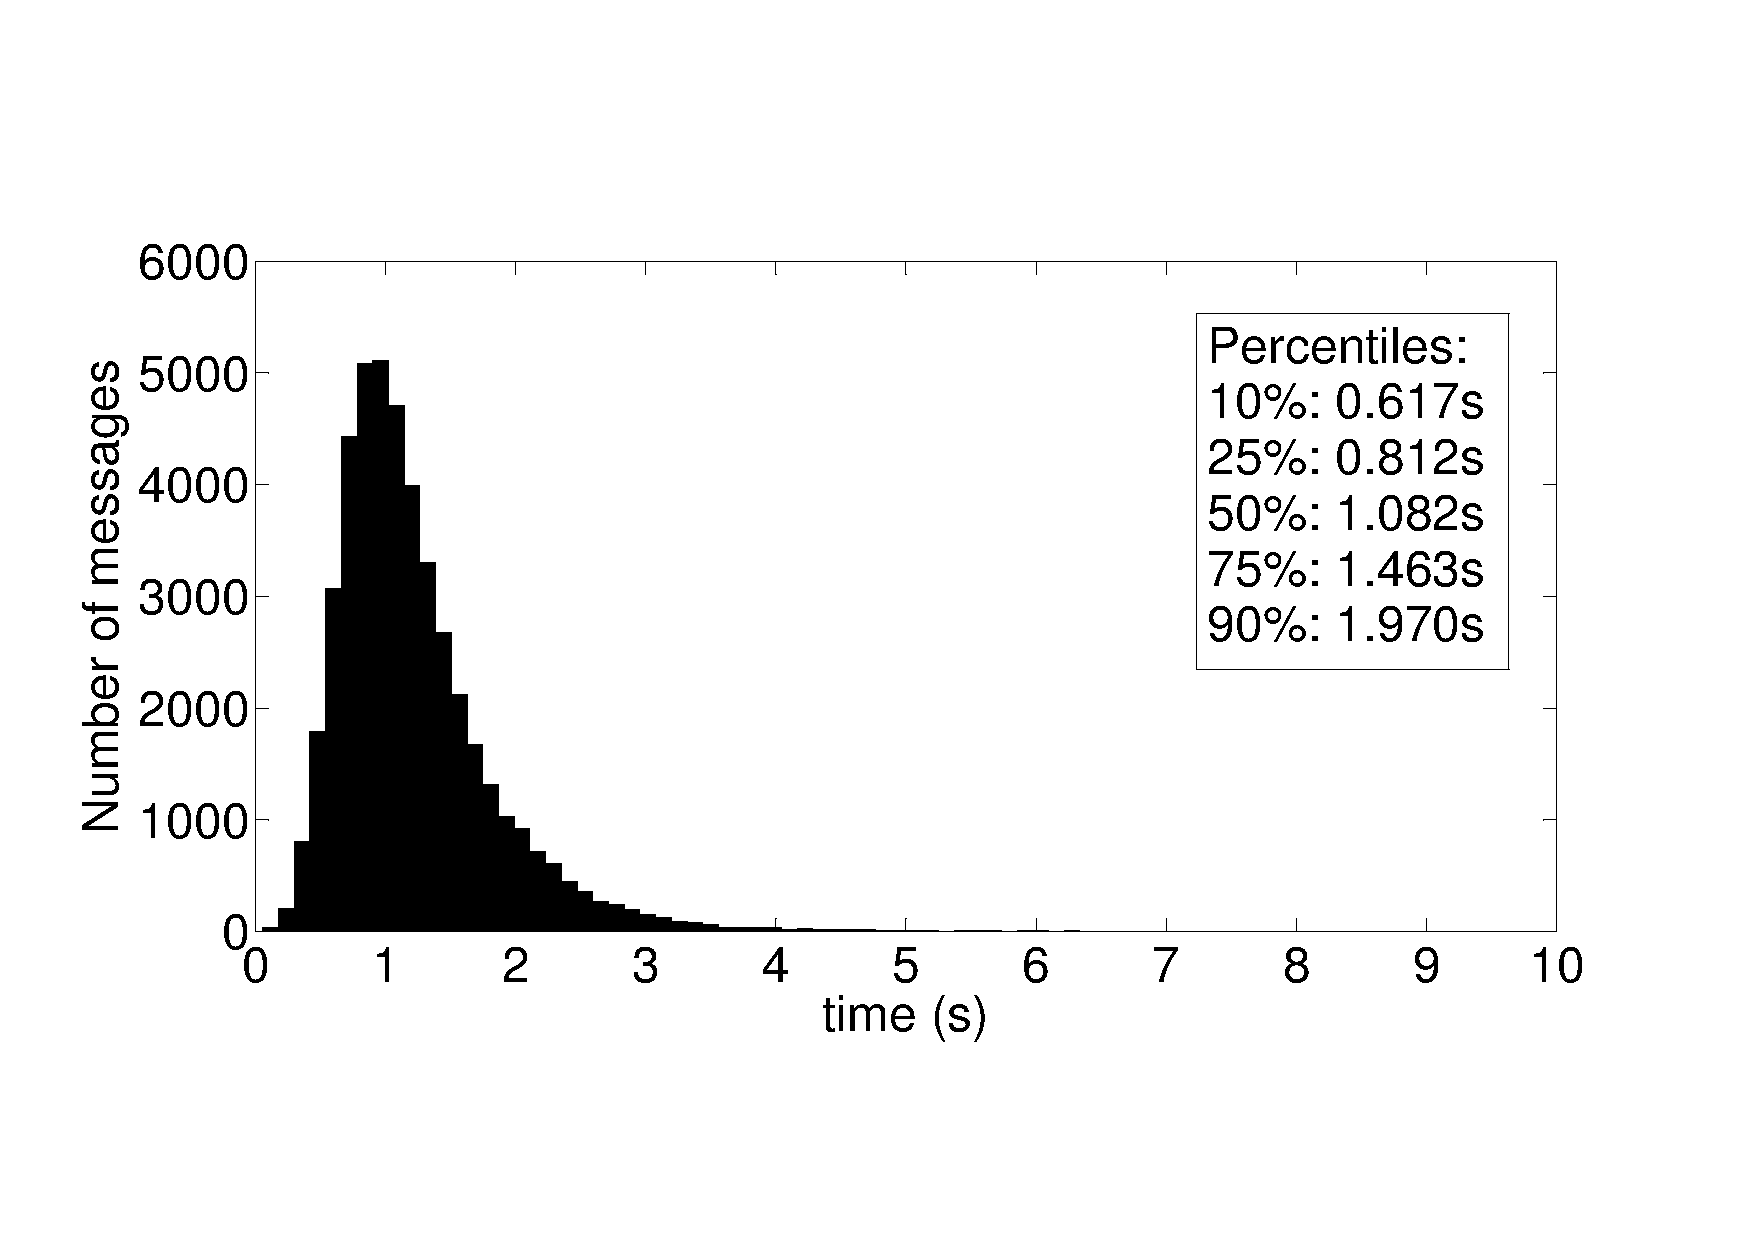
\includegraphics[clip=true, viewport=5mm 65mm 265mm 205mm, width=\columnwidth]{overlay_put_sf}
 \caption{Overlay storage responsiveness}
 \label{fig_overlay_put_sf}
\end{figure}
%
Figure \ref{fig_overlay_put_sf} shows that to store an object in the overlay can take anywhere from 0.1 to 4 seconds.

\begin{figure}[htbp]
 \centering
 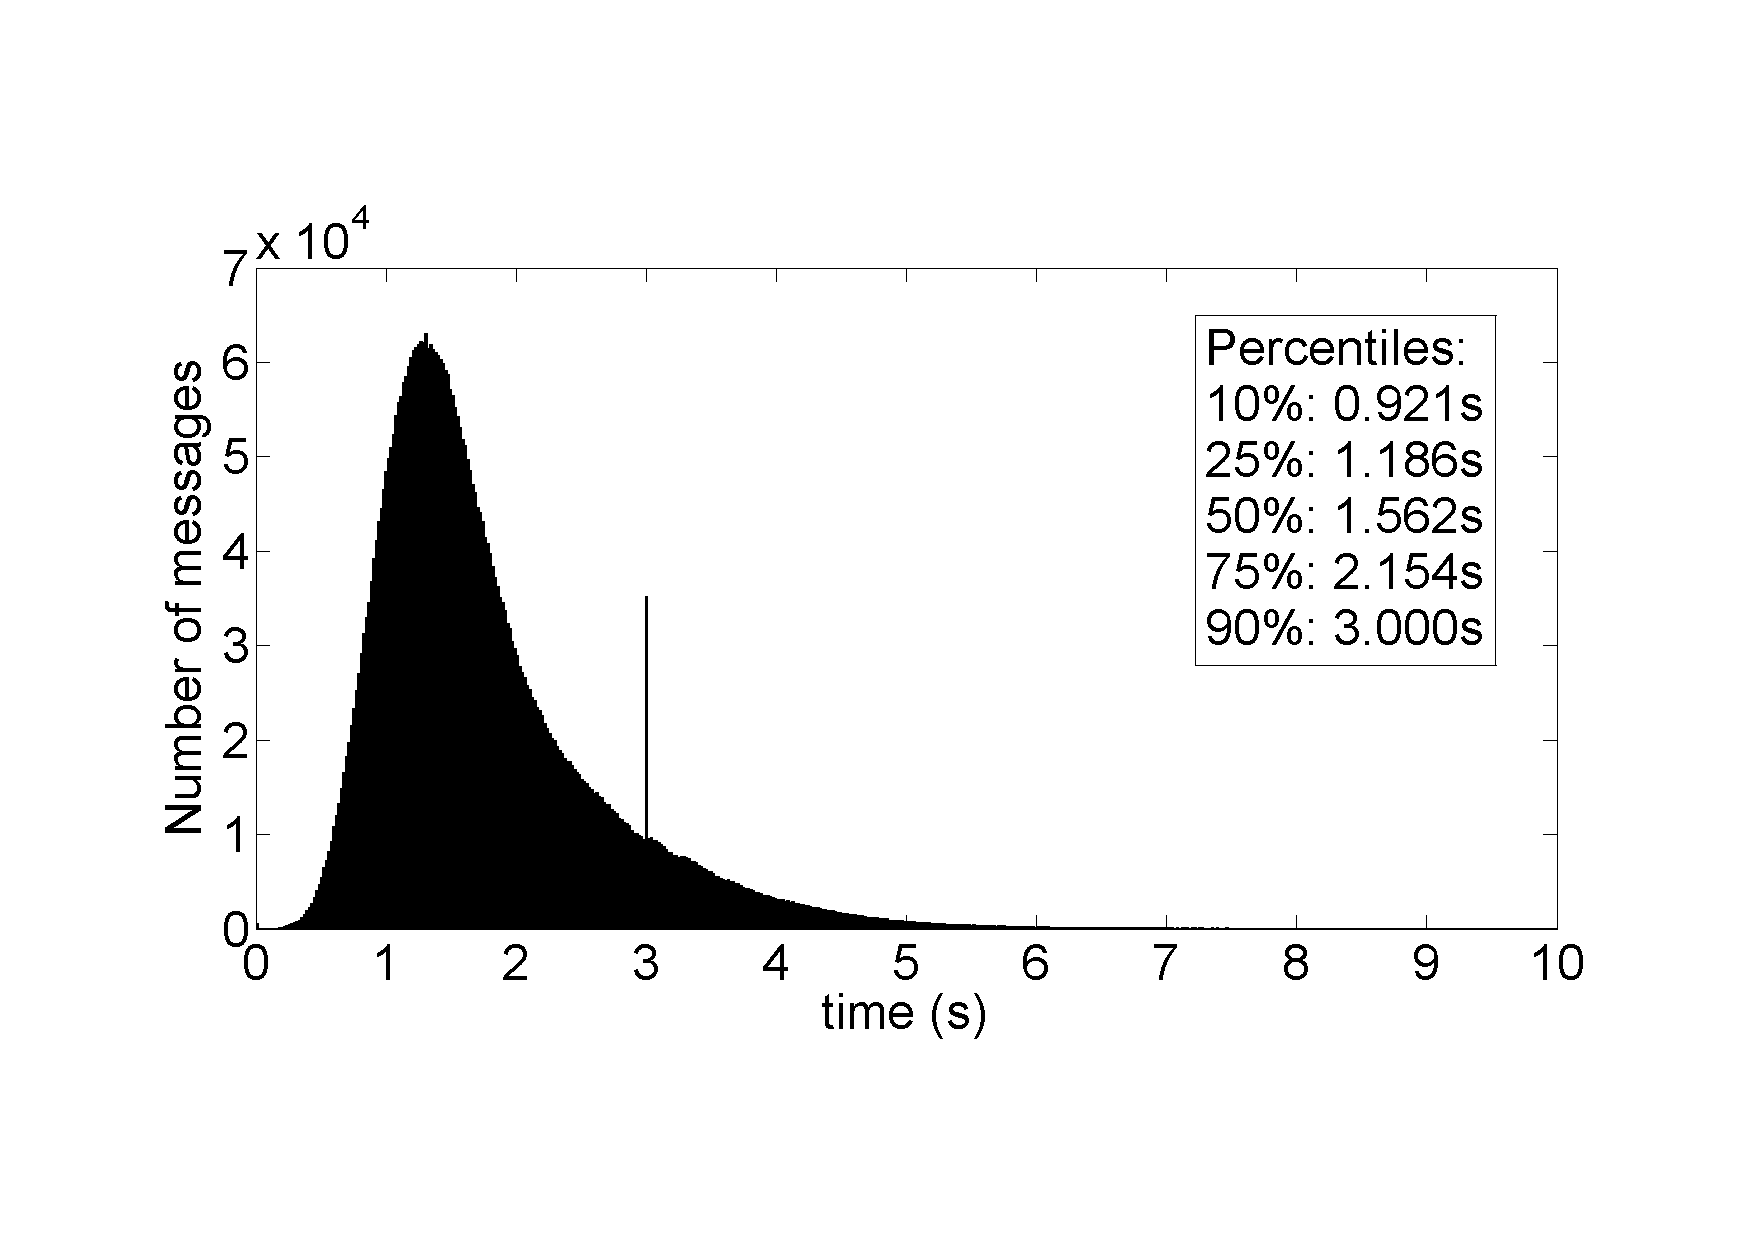
\includegraphics[clip=true, viewport=20mm 30mm 270mm 190mm, width=\columnwidth]{overlay_get_sf}
 \caption{Overlay retrieval responsiveness}
 \label{fig_overlay_get_sf}
\end{figure}
%
Figure \ref{fig_overlay_get_sf} shows that to retrieve an object from the overlay can take anywhere from 0.1 to 6 seconds. Figure \ref{fig_overlay_get_sf} also shows a spike at 3 seconds, when overlay retrieval is performed. This means that a large number of requests take 3 seconds to complete. This is thought to be an artifact of Chord lookup performance due to timeouts as set up in the Oversim simulation.

Overlay storage and retrieval has a high standard deviation when compared to group storage and retrieval as will be shown in the next sections.


\subsection{Group storage}
\label{group_storage_eval}

\subsubsection{Fast storage}
\label{group_put_f_fp}

Figure \ref{fig_group_put_fp} shows the distribution of group storage for fast storage.

\begin{figure}[htbp]
 \centering
 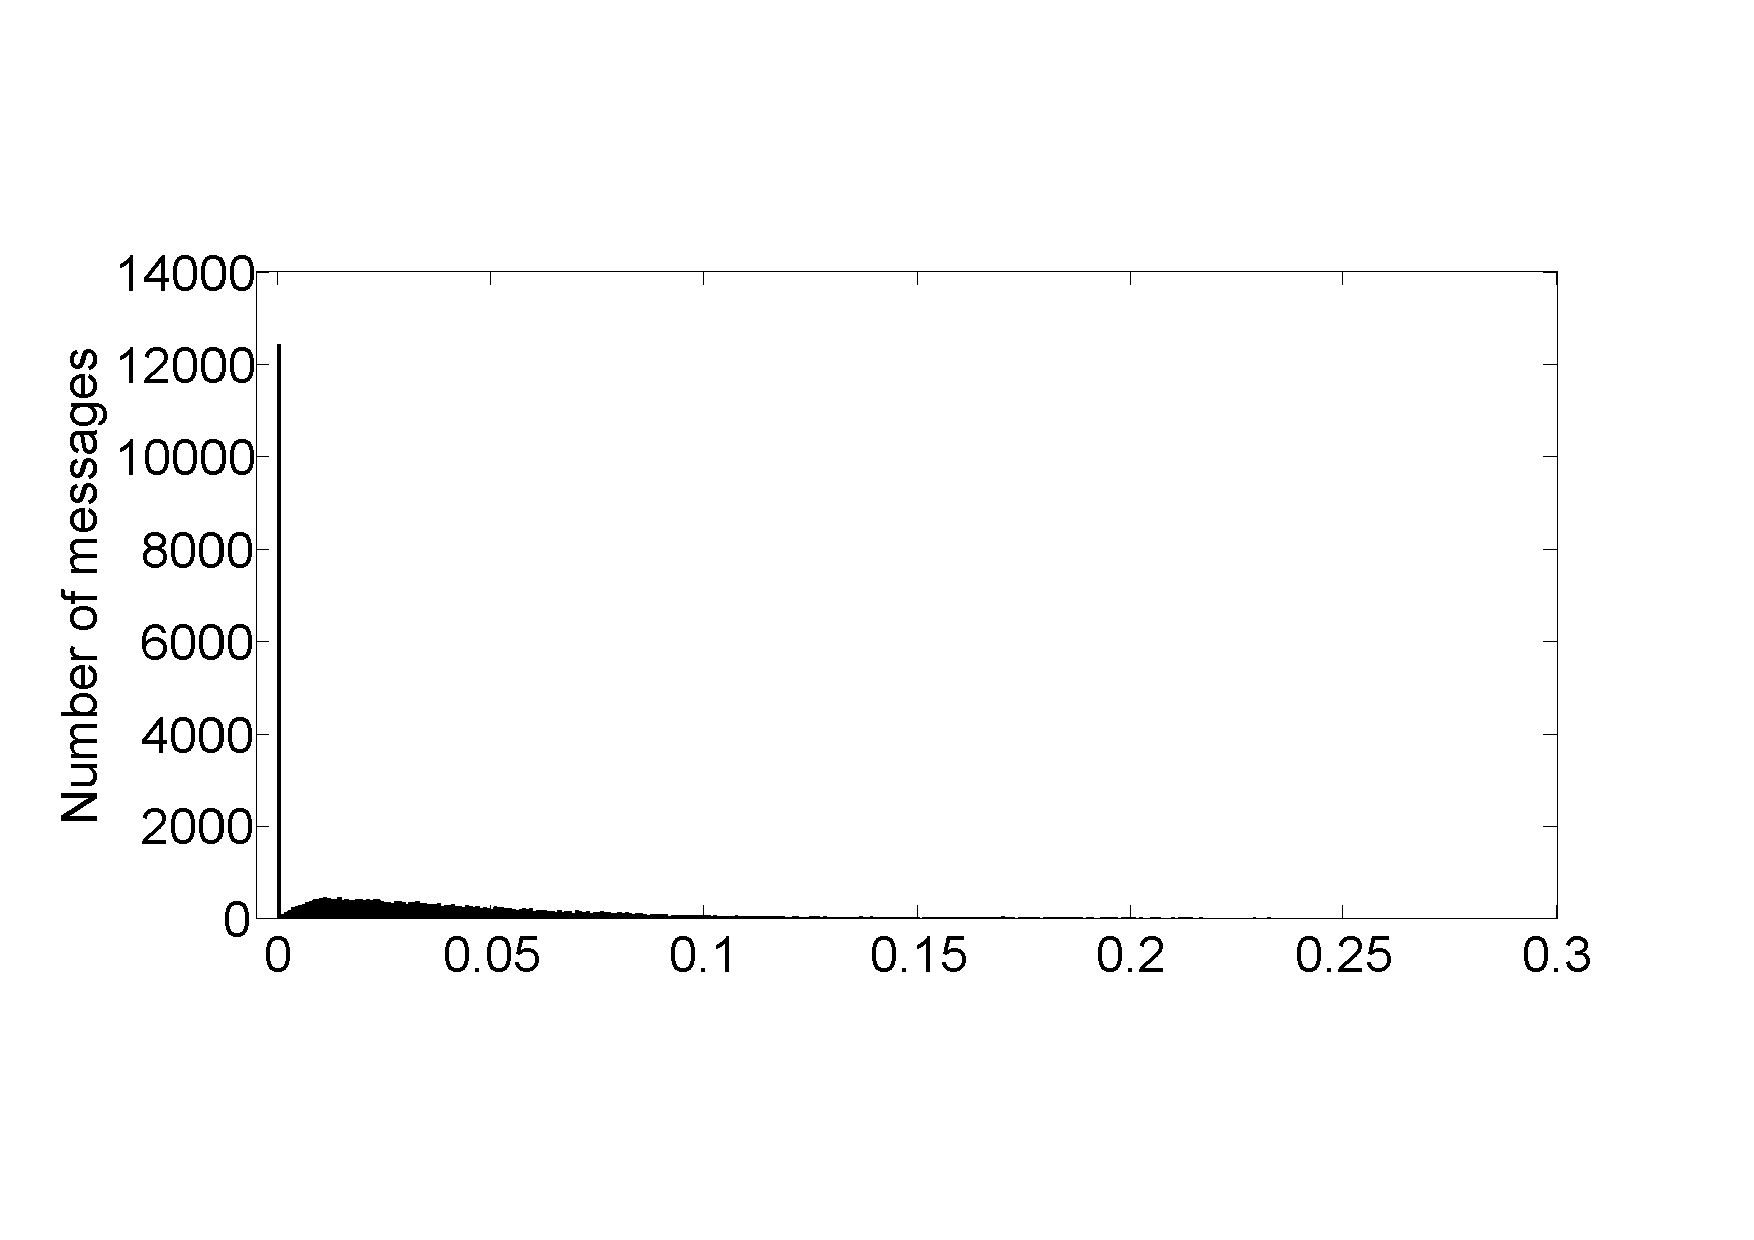
\includegraphics[clip=true, viewport=10mm 30mm 270mm 185mm, width=\columnwidth]{group_put_fp}
 \caption{Group storage responsiveness for fast storage}
 \label{fig_group_put_fp}
\end{figure}
%
Figure \ref{fig_group_put_fp} shows a high peak at close to zero seconds. This peak shows that a large number of storage requests have a small time compared to the rest of requests. These requests are the requests where the node generating the object is chosen to store the object. If the required number of replicas is high, compared to the group size, there is a high likelihood that the node originating the request will be chosen as a host node to the object. This is why there is such a large spike at close to zero.

It should be noted that the node that originally stored the object does not have local access to the object. Only other nodes that did not originally store the object may have access to local copies.

Apart from the spike, Figure \ref{fig_group_put_fp} also shows that the responsiveness is distributed over a small range: from zero to 0.1 seconds.

\subsubsection{Safe storage}
\begin{figure}[htbp]
 \centering
 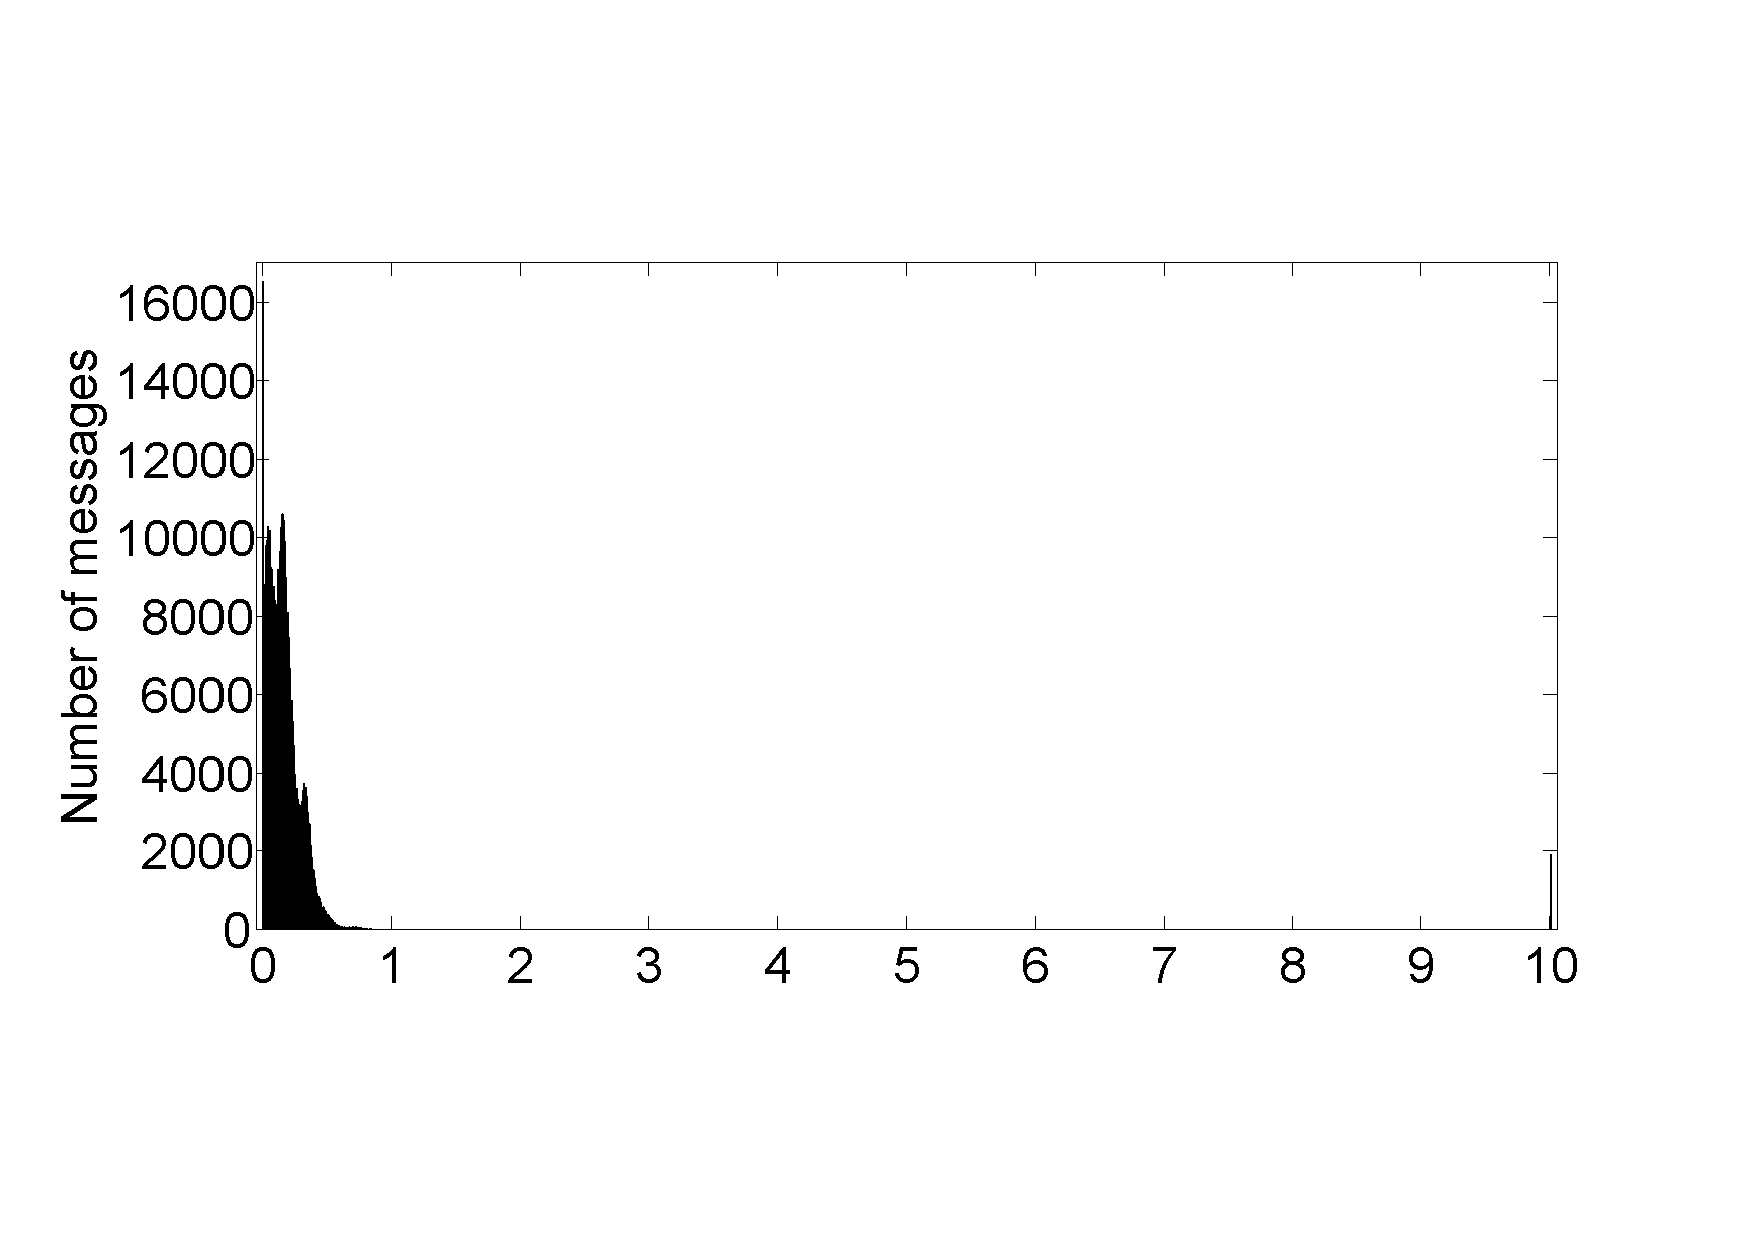
\includegraphics[clip=true, viewport=10mm 30mm 270mm 180mm, width=\columnwidth]{group_put_sf}
 \caption{Group storage responsiveness for safe storage}
 \label{fig_group_put_sf}
\end{figure}
%
Figure \ref{fig_group_put_sf} shows the responsiveness distribution for safe storage. Because safe storage is slower than fast storage, the mean response time is longer. The maximum and minimum responsiveness values are also greater than for fast storage: from zero to 0.8 seconds. This is still smaller than the range of overlay storage values.

Figure \ref{fig_group_put_sf} also contains a spike at 10s. This is due to the storage timeout being set to 10s. What should be noted is that these responsiveness graphs shows both success and failure responsiveness. In other words, it shows how quickly a response is received, even if that response is a failure. The responses received from 10 s are all failures, where no response was received from the destination node and an internal timeout occurred.

\subsection{Group retrieval}
\subsubsection{Fast retrieval}
\begin{figure}[htbp]
 \centering
 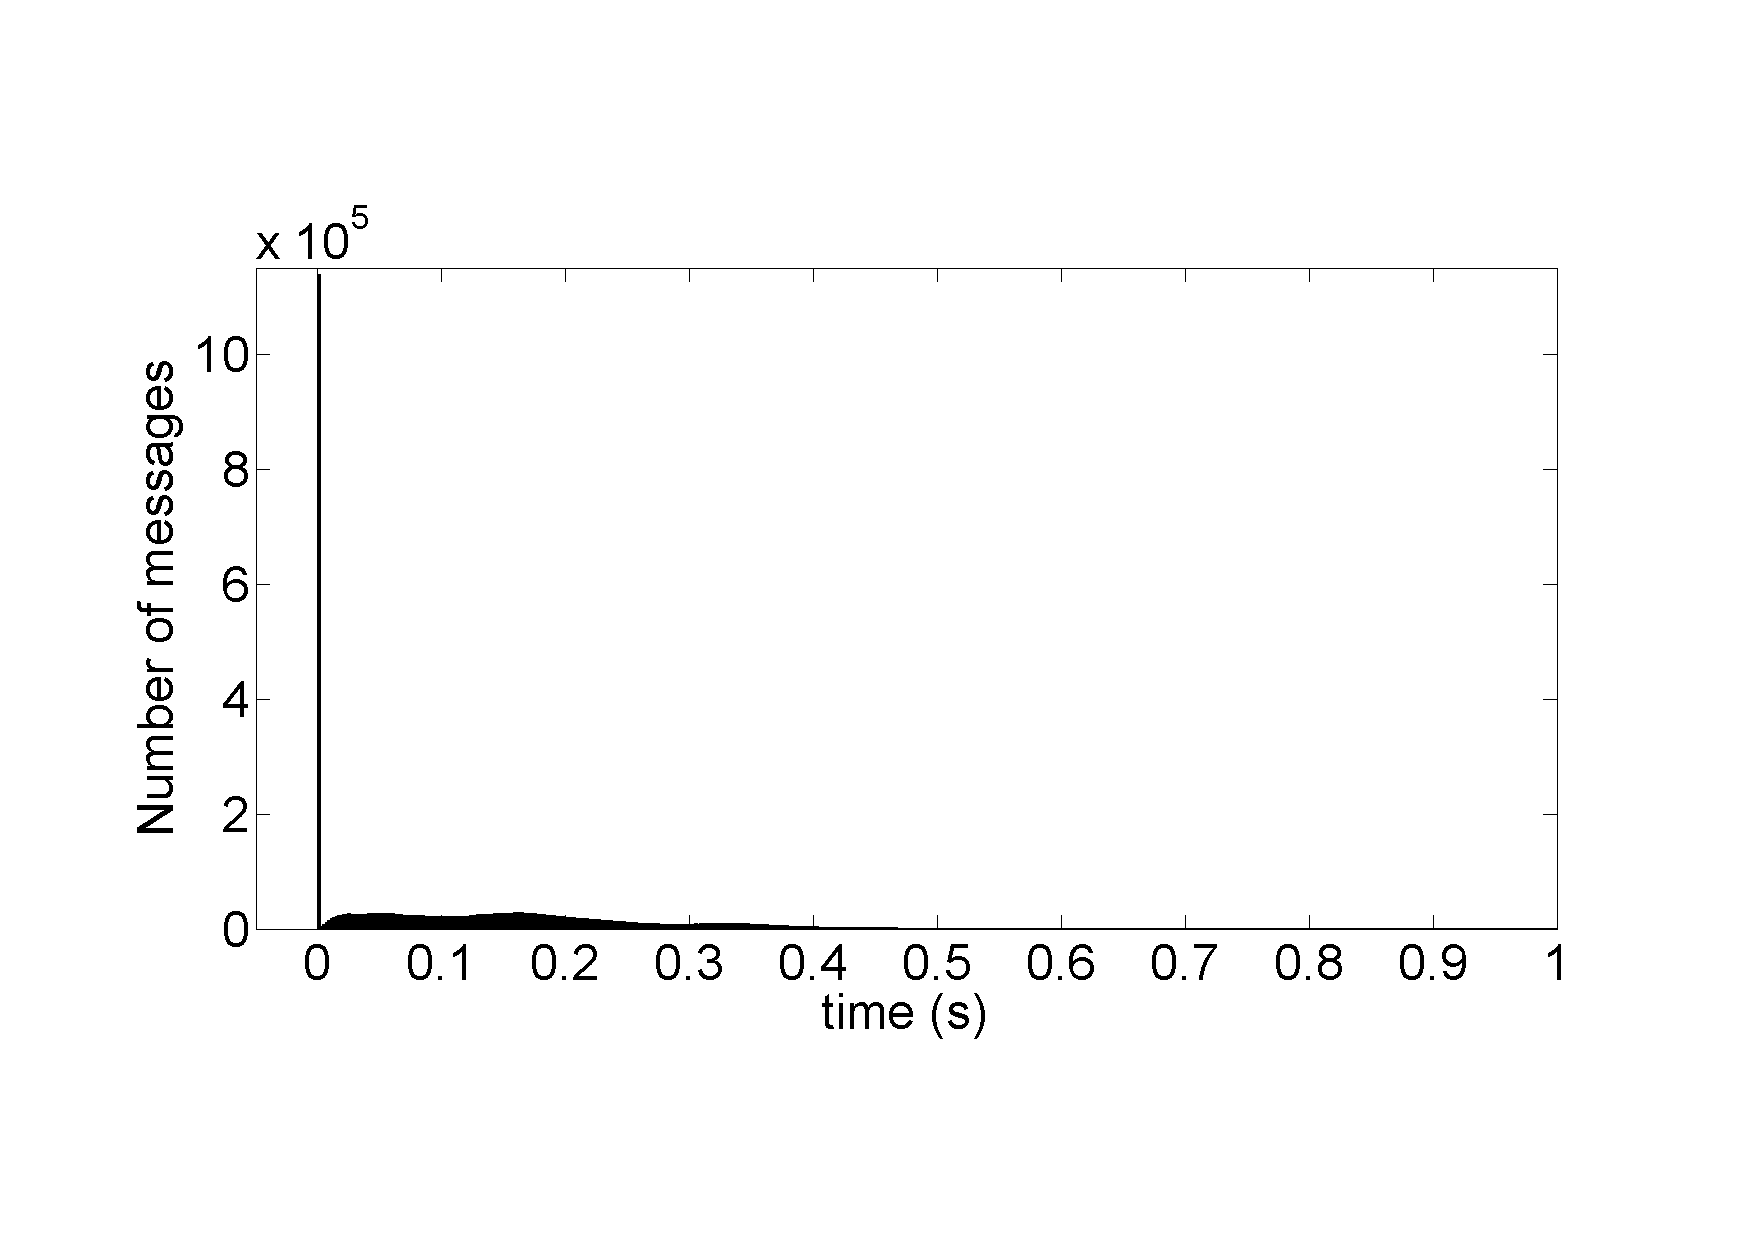
\includegraphics[clip=true, viewport=20mm 30mm 265mm 180mm, width=\columnwidth]{group_get_sf}
 \caption{Group retrieval responsiveness for fast retrieval}
 \label{fig_group_get_sf}
\end{figure}
%
Figure \ref{fig_group_get_sf} shows group retrieval responsiveness for fast retrieval. This type of retrieval also shows a spike at zero seconds due to nodes requesting objects from the network and those objects being found in the locally stored root object store. Because of the high number of replicas compared to the average group size used in the simulation, many of the requests can be locally served, which greatly increases responsiveness.

\begin{figure}[htbp]
 \centering
 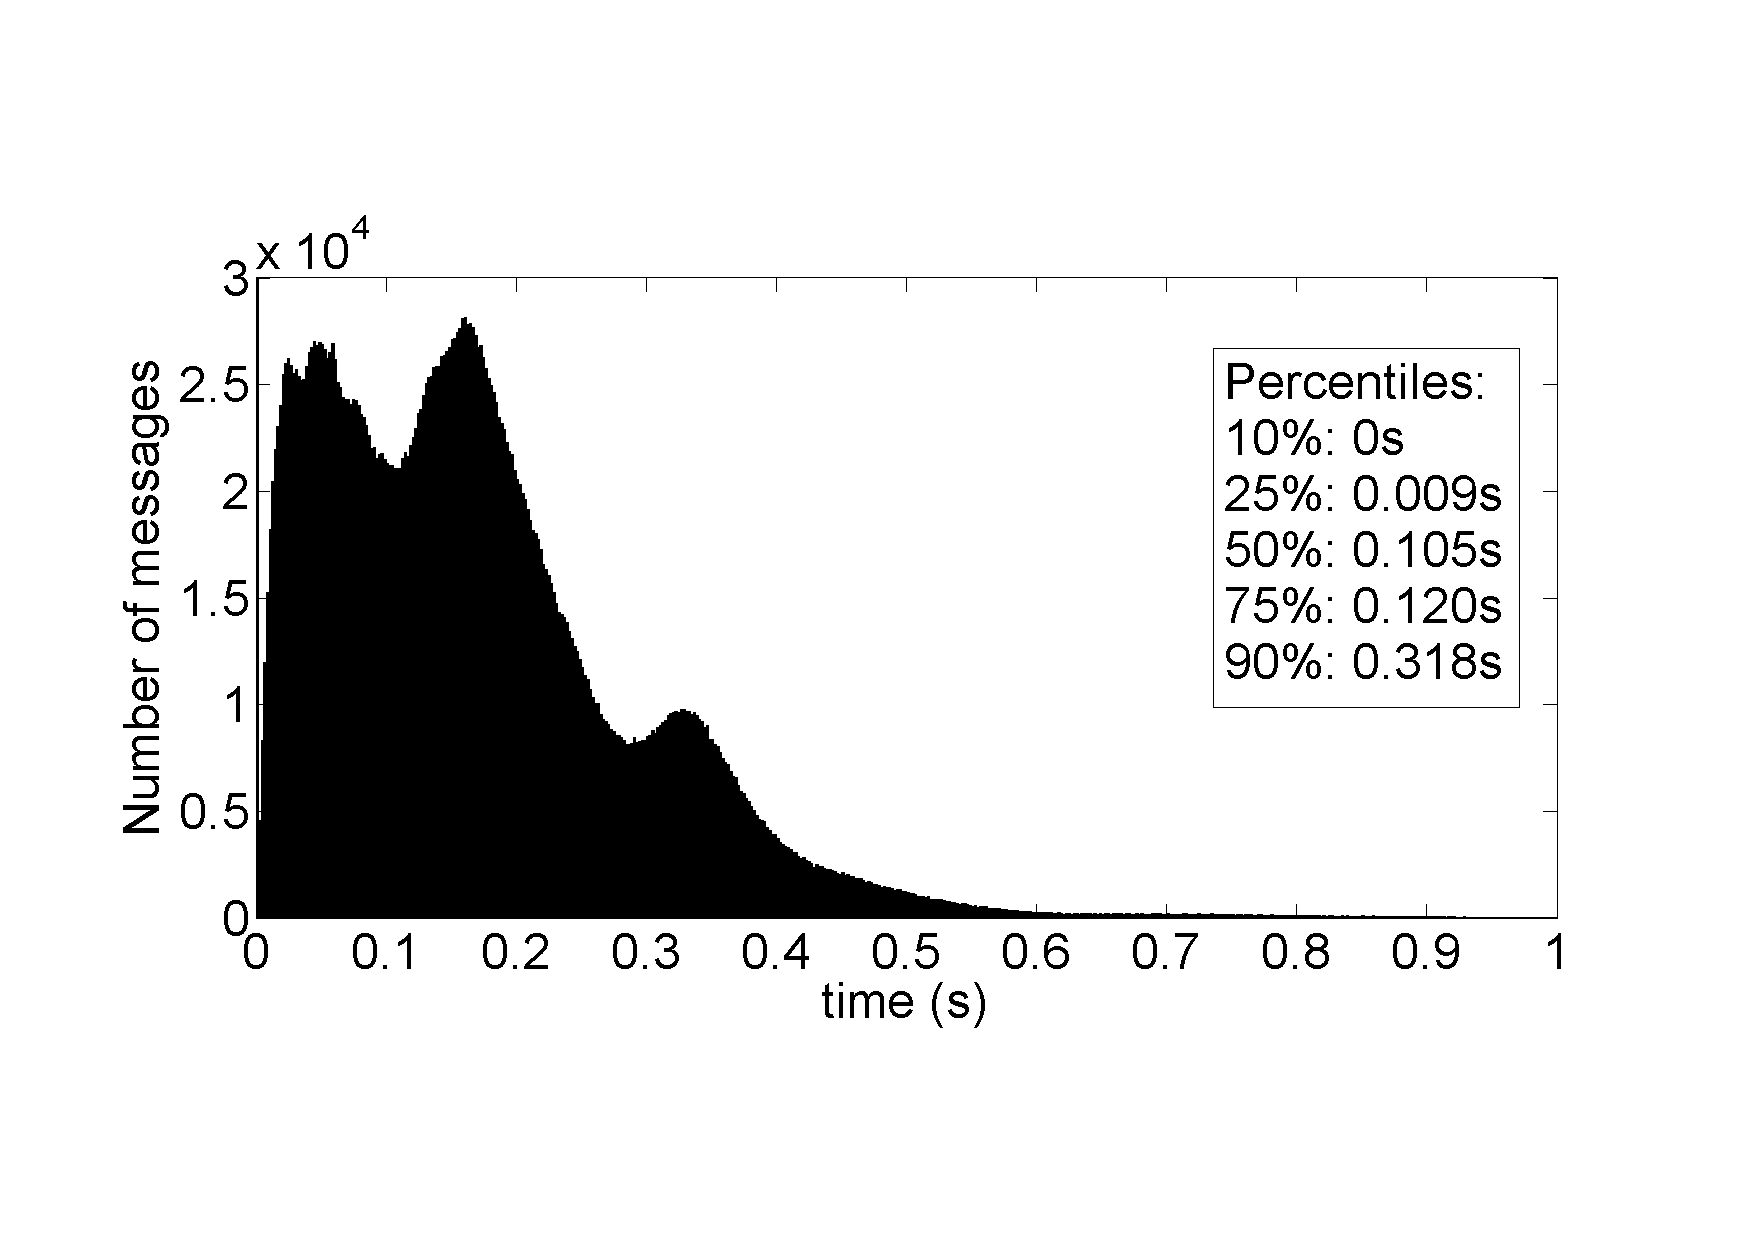
\includegraphics[clip=true, viewport=20mm 30mm 265mm 180mm, width=\columnwidth]{group_get_zoom_sf}
 \caption{Enlarged view of the group retrieval responsiveness for fast retrieval}
 \label{fig_group_get_zoom_sf}
\end{figure}
%
Figure \ref{fig_group_get_zoom_sf} is an enlarged view of Figure \ref{fig_group_get_sf}, to more clearly show the multimodal responsiveness. This figure also shows multiple peaks, which is shown to be an artifact of the underlying physical layer in Section \ref{lan_retrieval}.

The figure shows that fast group retrieval responsiveness varies from zero to 0.9 seconds.

\subsubsection{Parallel retrieval}
\begin{figure}[htbp]
 \centering
 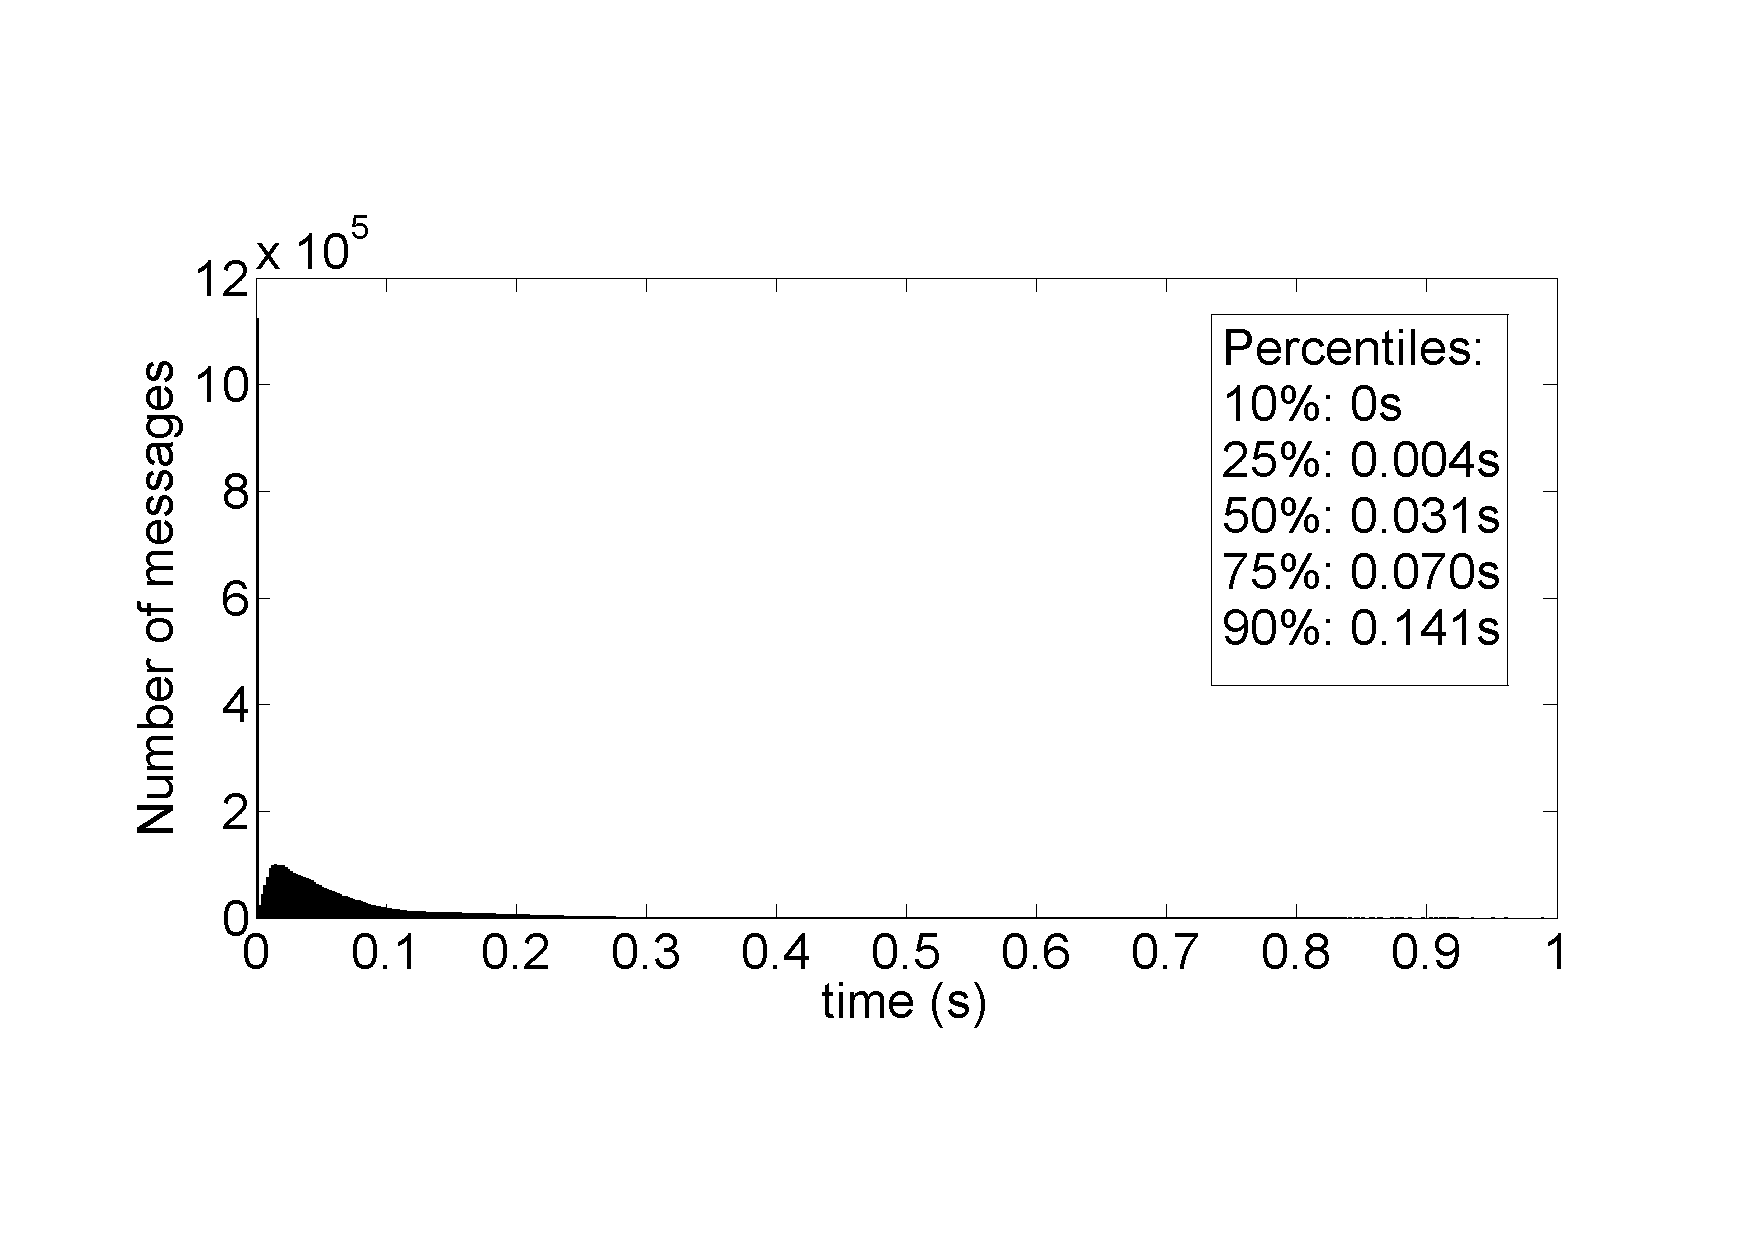
\includegraphics[clip=true, viewport=20mm 30mm 265mm 180mm, width=\columnwidth]{group_get_fp}
 \caption{Group retrieval responsiveness for parallel retrieval}
 \label{fig_group_get_fp}
\end{figure}

\begin{figure}[htbp]
 \centering
 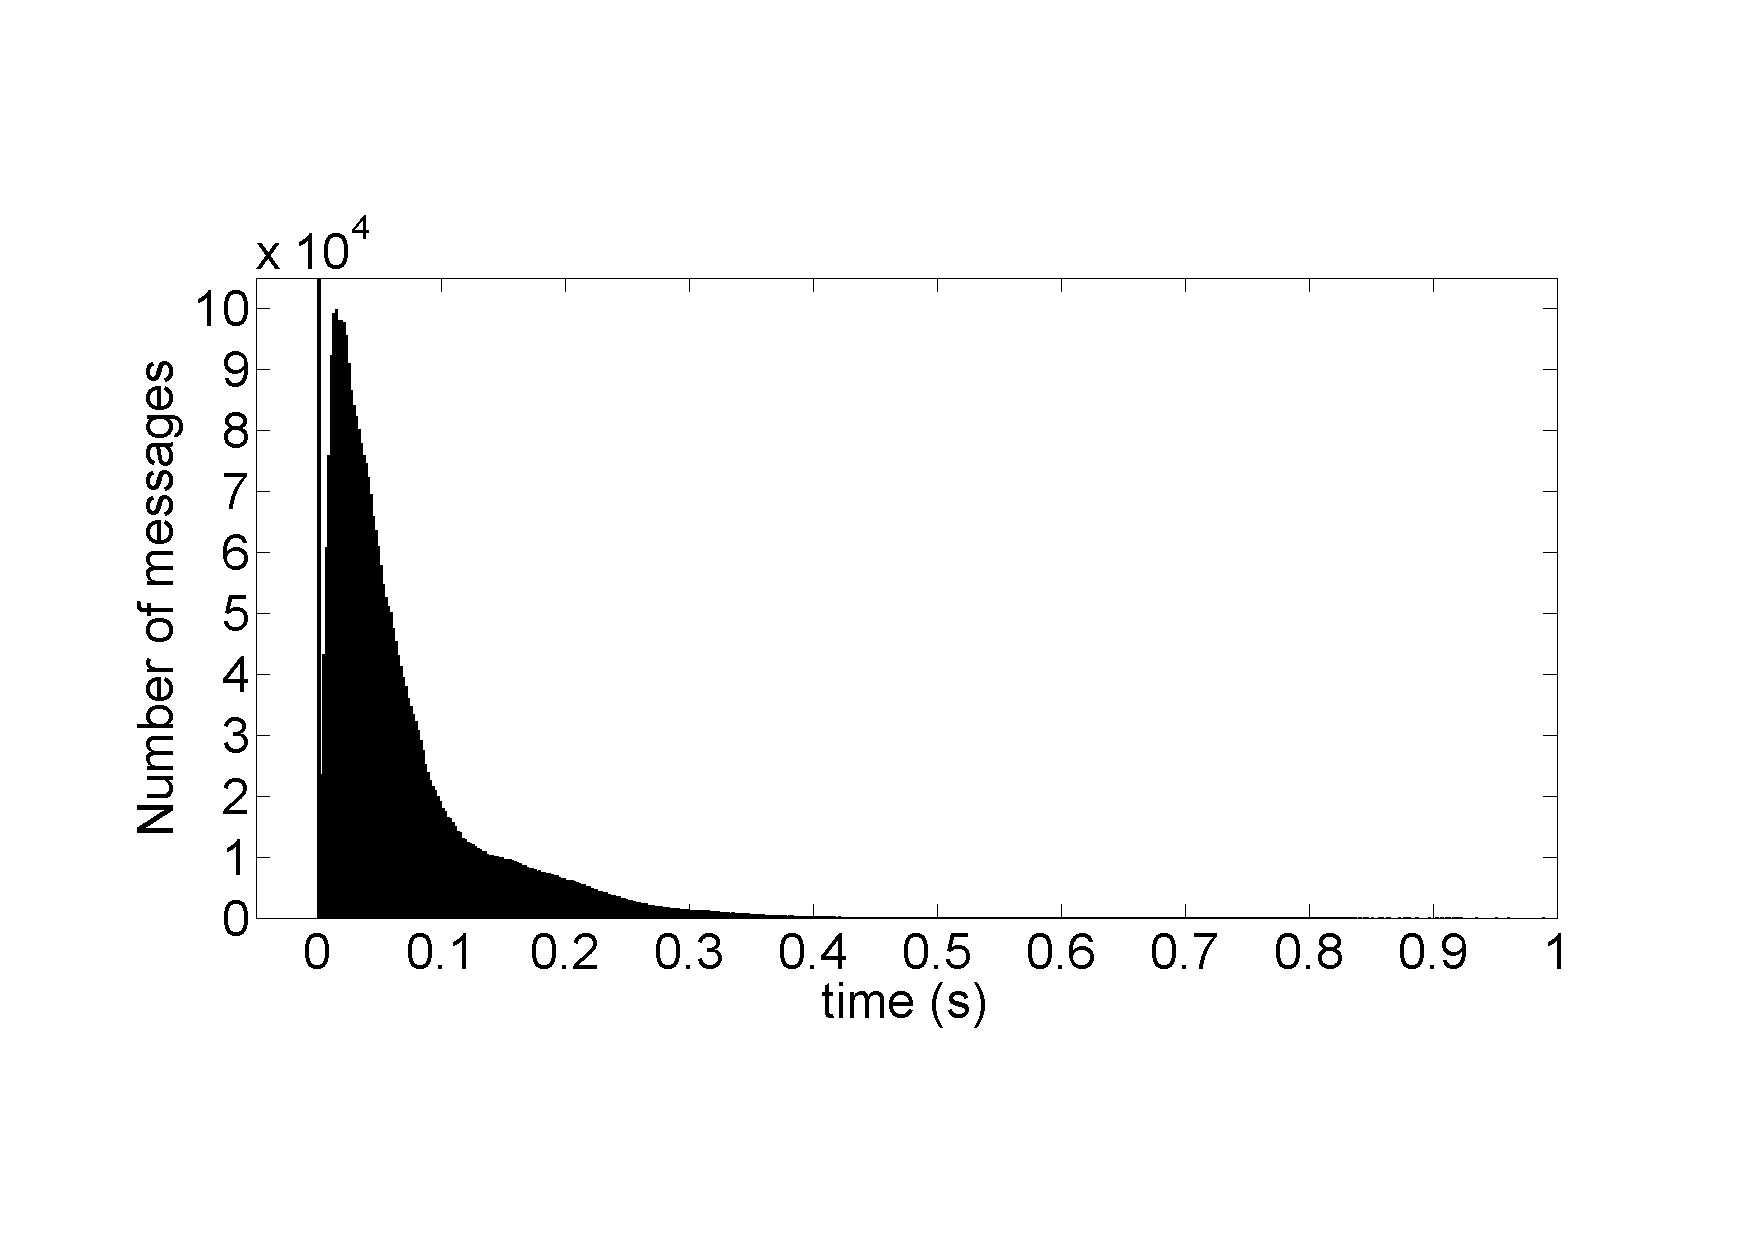
\includegraphics[clip=true, viewport=20mm 30mm 265mm 180mm, width=\columnwidth]{group_get_zoom_fp}
 \caption{Enlarged view of the group retrieval responsiveness for parallel retrieval}
 \label{fig_group_get_zoom_fp}
\end{figure}
%
Figure \ref{fig_group_get_fp} shows group retrieval responsiveness for parallel retrieval. Figure \ref{fig_group_get_zoom_fp} shows the enlarged view. Apart from the higher responsiveness, which is a result of multiple replicas queried and the fastest response being used (as previously explained in Section \ref{pithos_resp_rel_results}), parallel retrieval also has a smaller range of values: from zero to 0.4 seconds.

The shape of Figure \ref{fig_group_get_zoom_fp} differs from that of Figure \ref{fig_group_get_zoom_sf} due to the difference between selecting a single random node ($1/r$) in the group for retrieval, to selecting the fastest of $r$ nodes in the group for retrieval, where $r$ is the number of object replicas currently in the group.

\subsection{LAN performance}
\label{lan_retrieval}

Figures \ref{fig_group_put_sf} and \ref{fig_group_get_zoom_sf} show peaks (local maxima) that were suspected to be caused by the underlying network. To verify this, another simulation run is performed where the coordinate-based system used in Oversim is replaced by fixed 1ms delay links with 0.1\% jitter. The purpose of this is to show that group storage does indeed have the expected number of hops for a fully connected network and that the multimodal behaviour is a function of the distance of peers in the physical network layer. It should also be verified that the responsiveness of Pithos will improve if the physical layer latencies are reduced.

\begin{figure}[htbp]
 \centering
 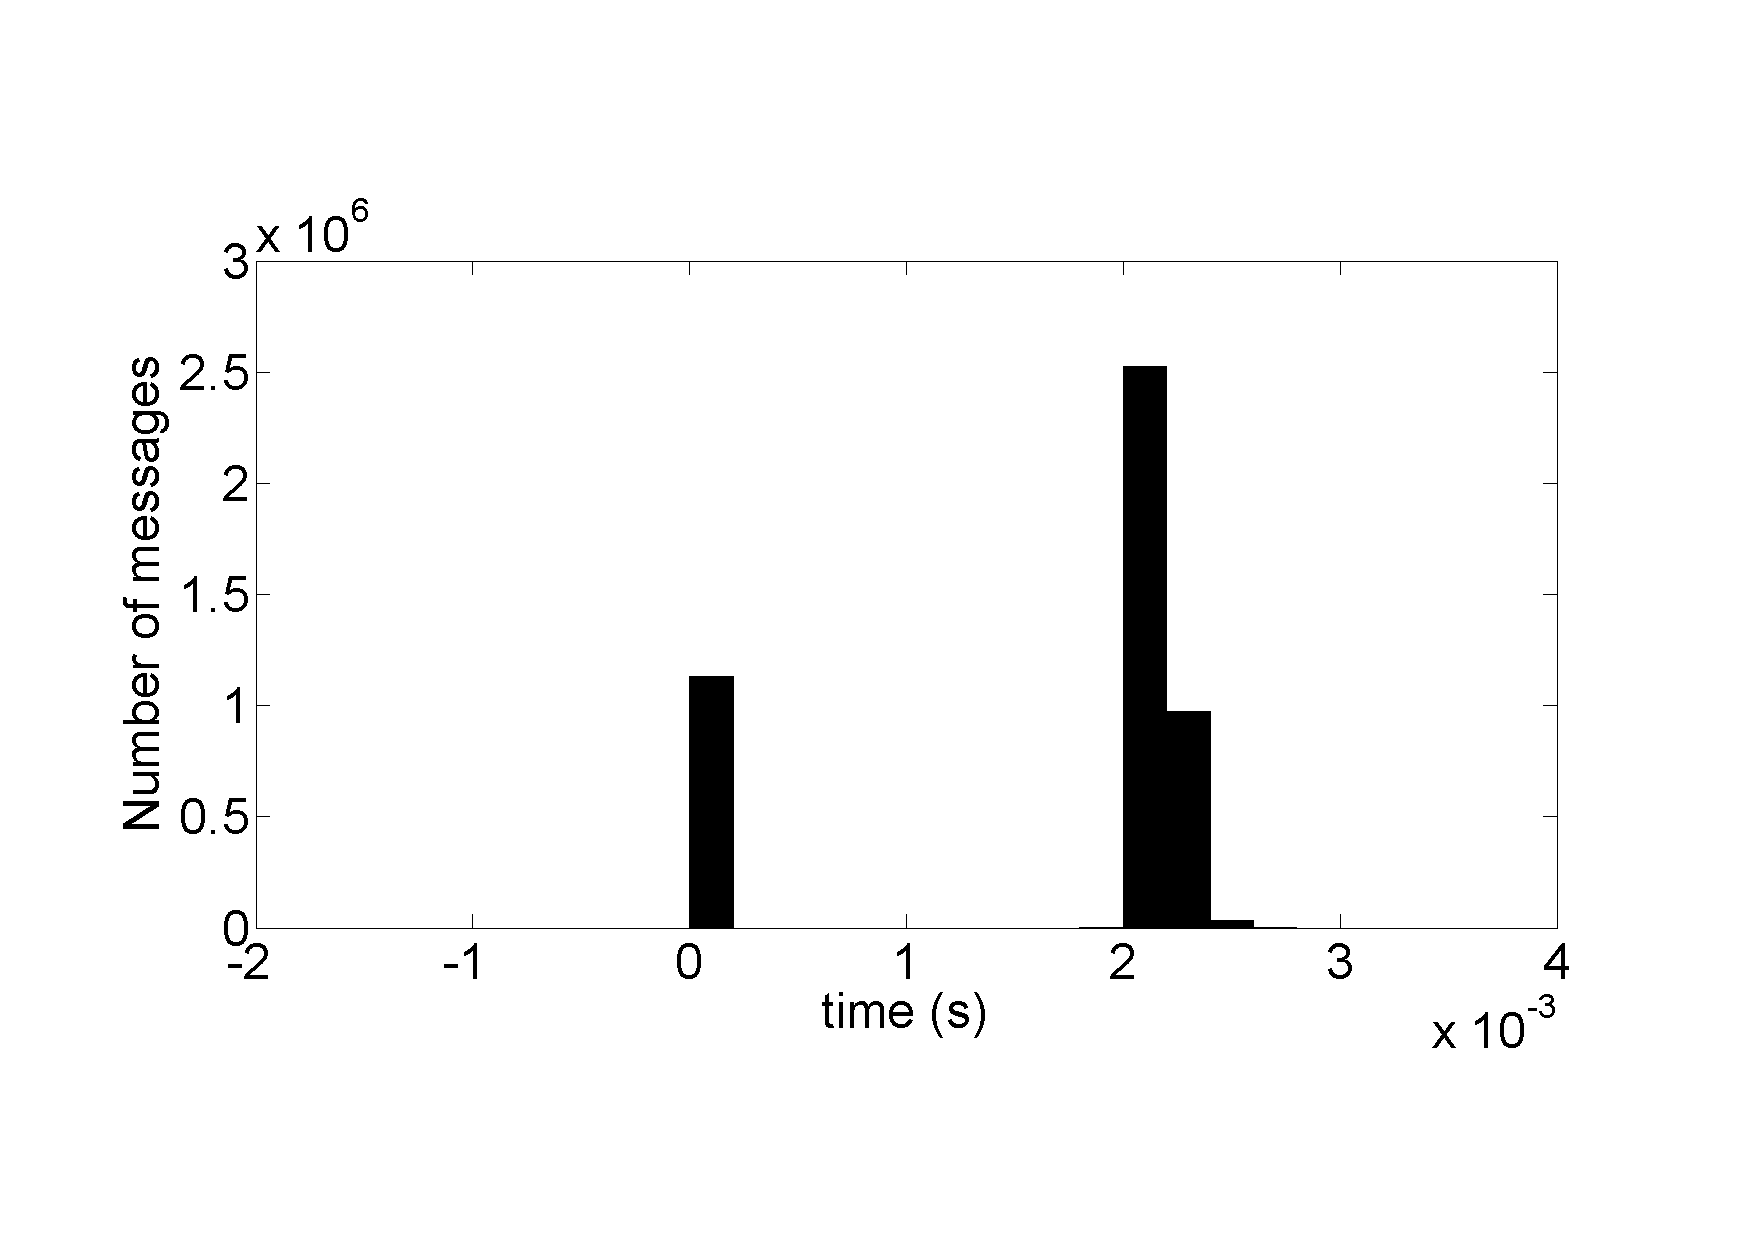
\includegraphics[clip=true, viewport=20mm 30mm 265mm 180mm, width=\columnwidth]{group_get_lan}
 \caption{Group retrieval responsiveness for fast storage and fast retrieval, running on a 1ms underlay network.}
 \label{fig_group_get_lan}
\end{figure}
%
Figure \ref{fig_group_get_lan} shows group retrieval performance for fast storage and fast retrieval, running on a 1ms underlay network. This figure shows the same operation shown in Figure \ref{fig_group_get_zoom_sf}, but for the underlay being a fixed 1ms underlay, instead of a coordinate-based underlay.

Two main spikes are seen in the figure, one at 0s and another at 2ms. The second spike is surrounded by the 0.1\% jitter, but the first spike contains no jitter, since no network message is sent out for the local storage. There are no other measured times. This is what is expected from group storage, since every request in group storage is either zero hops or two hops. For two hops, one hop is required to send the request, and another to receive the response, which gives $2\times 1 ms = 2 ms$. The zero hops case was explained in Section \ref{group_put_f_fp}.

No additional spikes are perceived, as opposed to the peaks seen earlier. The mean group storage performance has improved to 1.6ms, from the 192ms for the coordinate-based underlay network.

\subsection{Overall storage}

\subsubsection{Fast storage}
After having presented the separate responsiveness profiles for overlay and group storage, the overall Pithos responsiveness is presented here which is a combination of the responsiveness profiles of the underlying group and overlay responsiveness.

\begin{figure}[htbp]
 \centering
 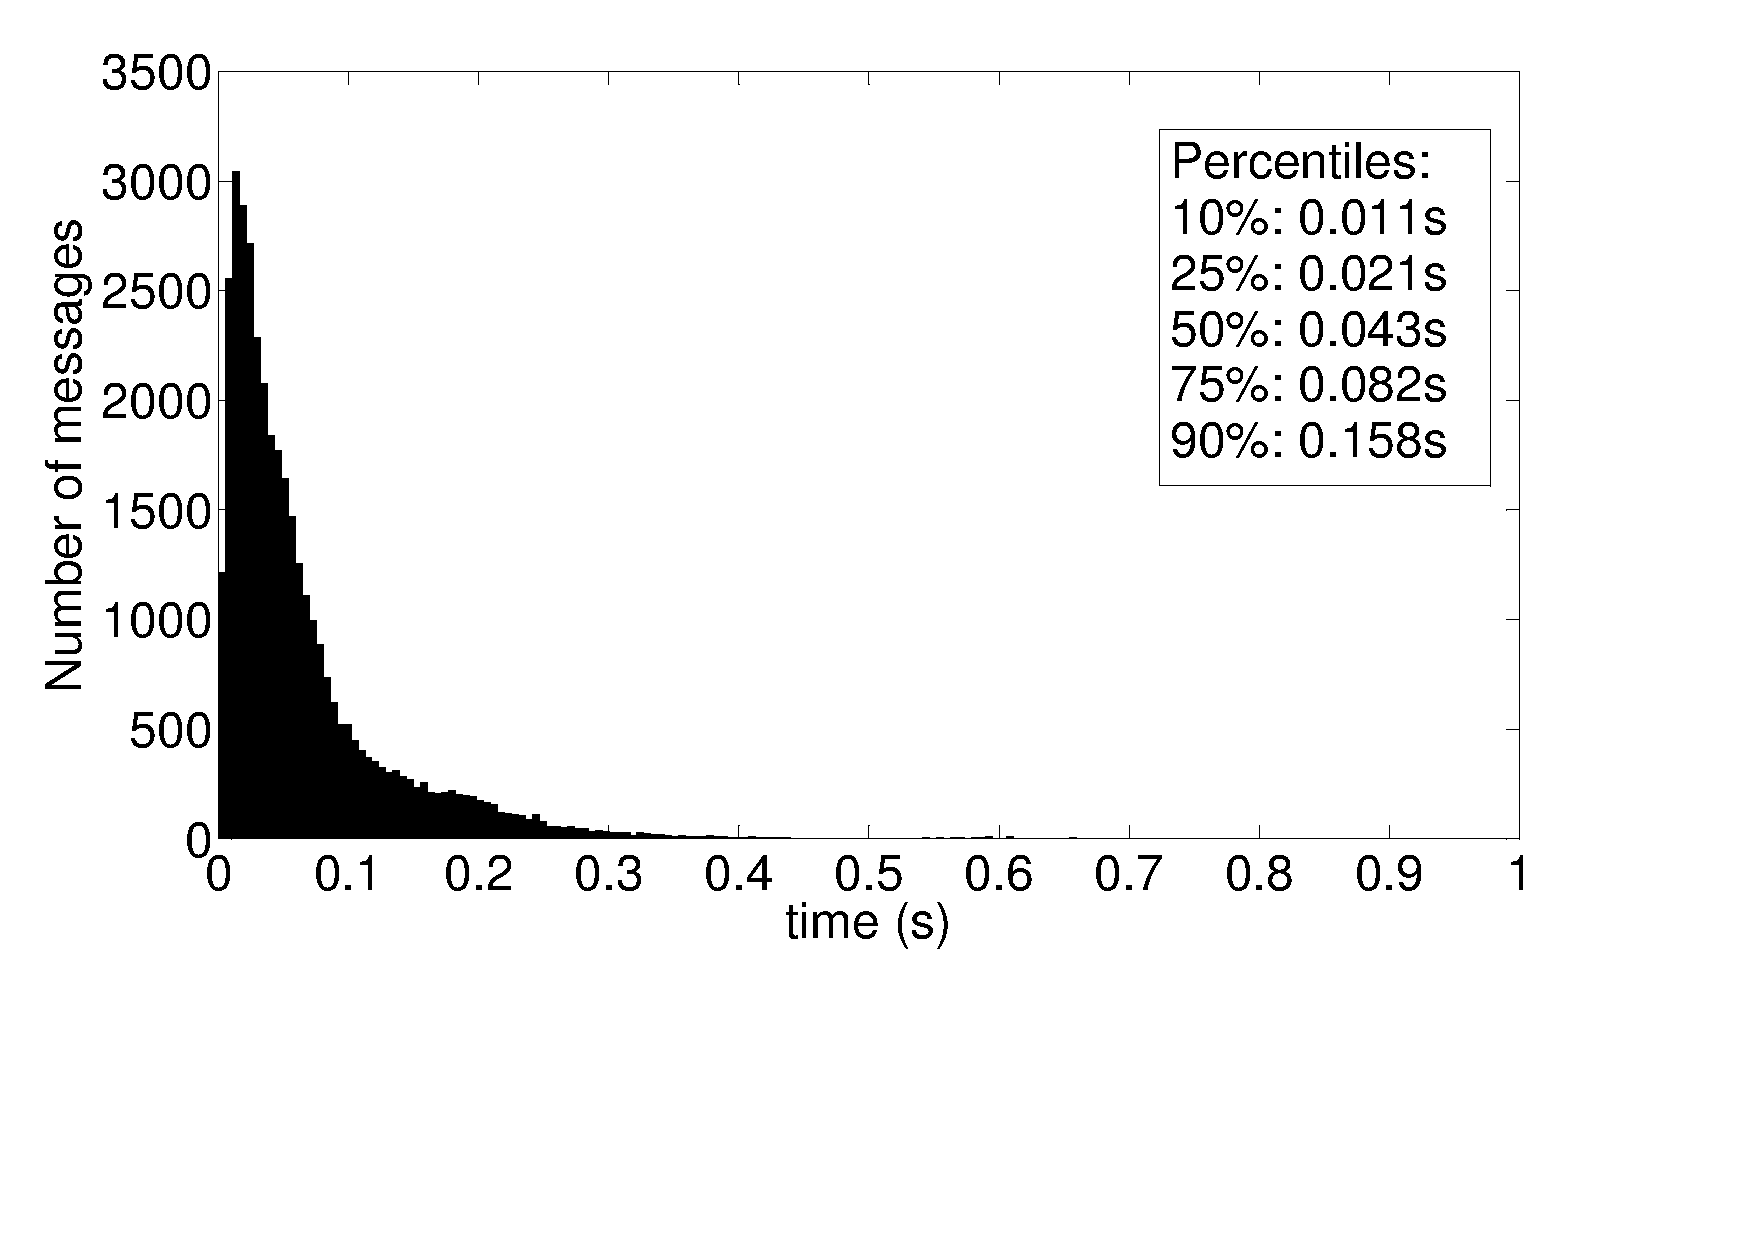
\includegraphics[clip=true, viewport=5mm 35mm 265mm 190mm, width=\columnwidth]{overall_put_ff}
 \caption{Overall storage responsiveness for fast storage}
 \label{fig_overall_put_ff}
\end{figure}
%
Figure \ref{fig_overall_put_ff} shows the overall storage responsiveness for fast storage. The shape is similar to that of Figure \ref{fig_group_get_zoom_fp}, a seemingly exponential distribution. The shape is derived from how fast storage tracks a success: the first successful storage response from group storage is sent to the higher layer, effectively taking all responses and choosing the fastest one. Fast storage responsiveness is, therefore, exactly the same mechanism as with parallel retrieval, which is why the distributions look that same.

Fast storage responsiveness ranges from zero to 0.3 seconds.

\subsubsection{Safe storage}
\begin{figure}[htbp]
 \centering
 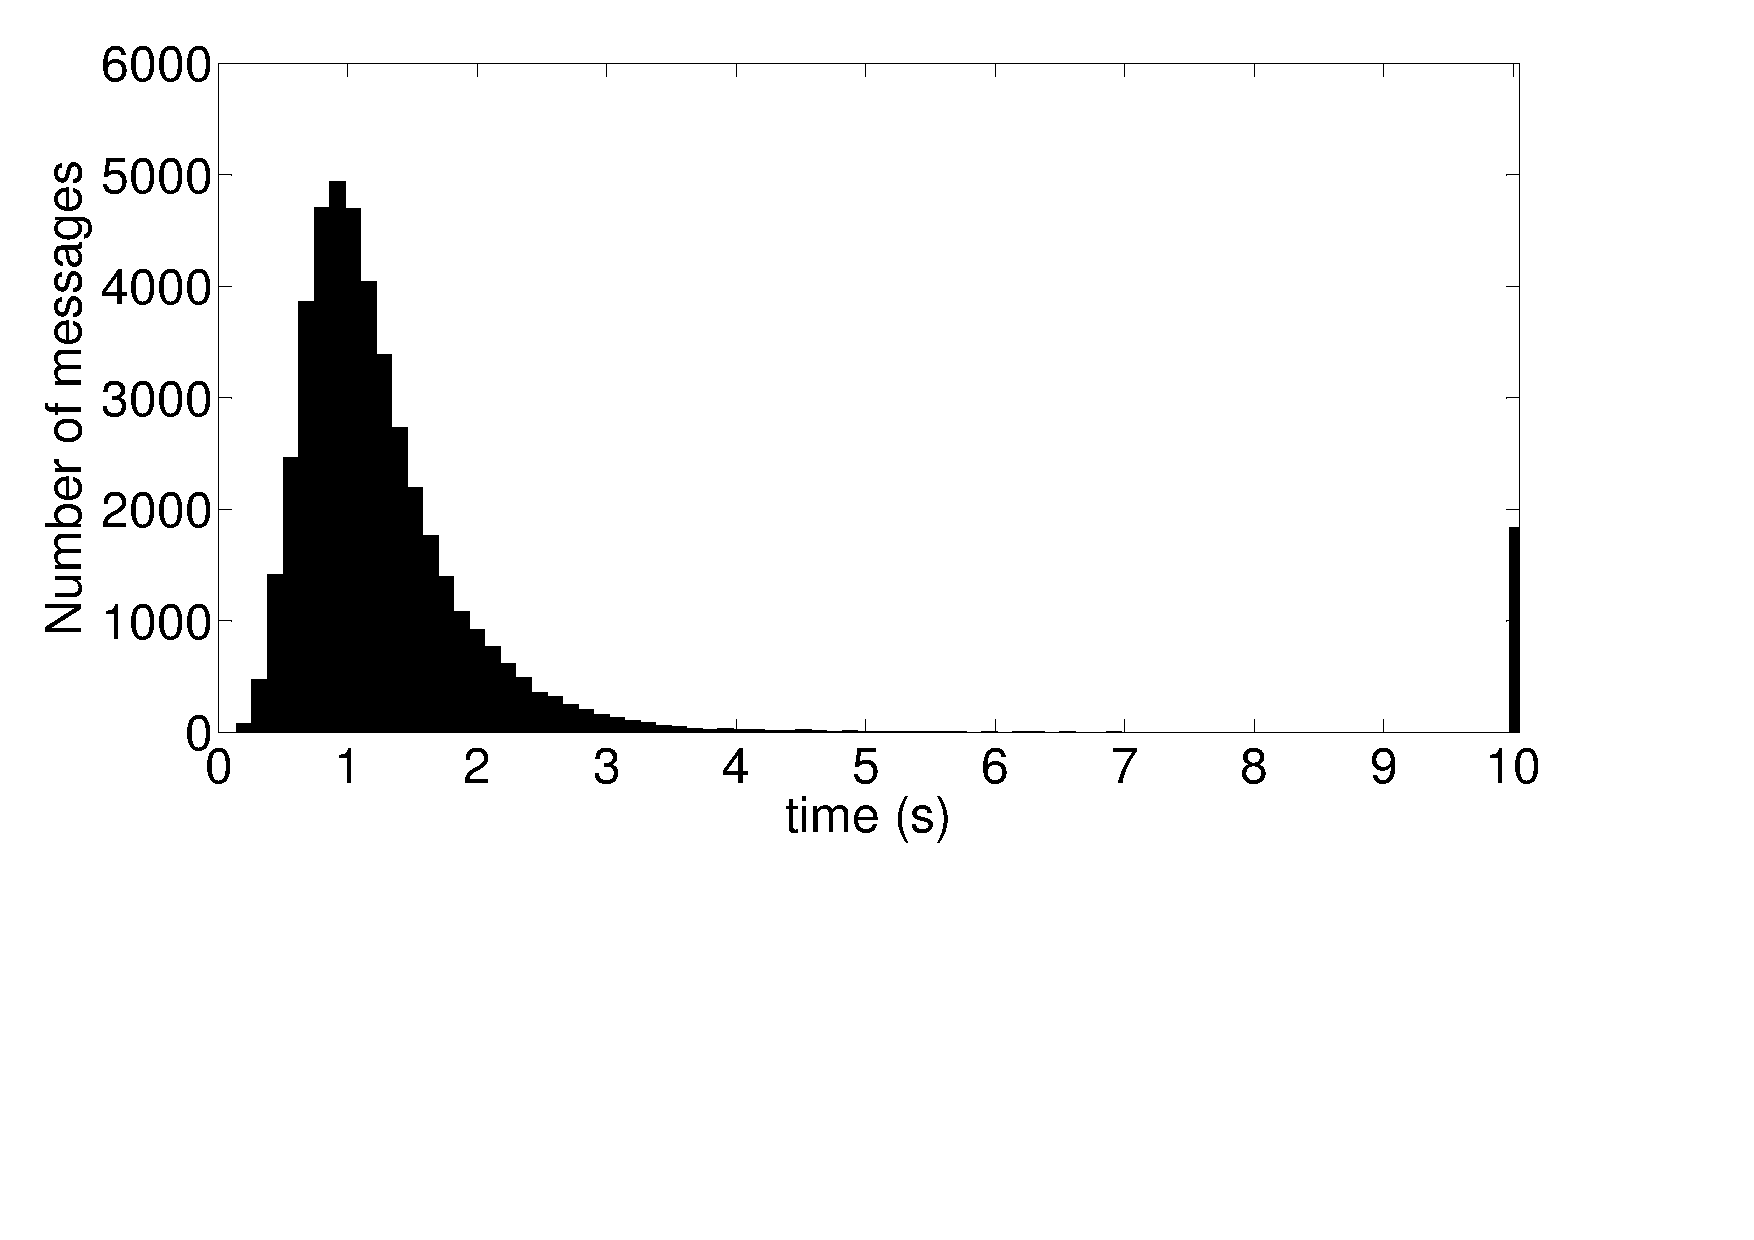
\includegraphics[clip=true, viewport=5mm 60mm 265mm 205mm, width=\columnwidth]{overall_put_sf}
 \caption{Overall storage responsiveness for safe storage}
 \label{fig_overall_put_sf}
\end{figure}
%
Figure \ref{fig_overall_put_sf} shows the overall storage responsiveness for safe storage. Because a response is only sent when sufficiently many group responses have been received \emph{and} when the overlay response has been received, the shape of the distribution is identical to that of the overlay storage distribution, shown in Figure \ref{fig_overlay_put_sf}.

The reason why the shape has no correspondence to group storage responsiveness is because, as previously shown, overlay storage is always slower than group storage. Because safe storage always waits for the reply from the overlay storage module, its responsiveness is dominated by the responsiveness of overlay storage.

\subsection{Overall retrieval}
\subsubsection{Fast retrieval}
\begin{figure}[htbp]
 \centering
 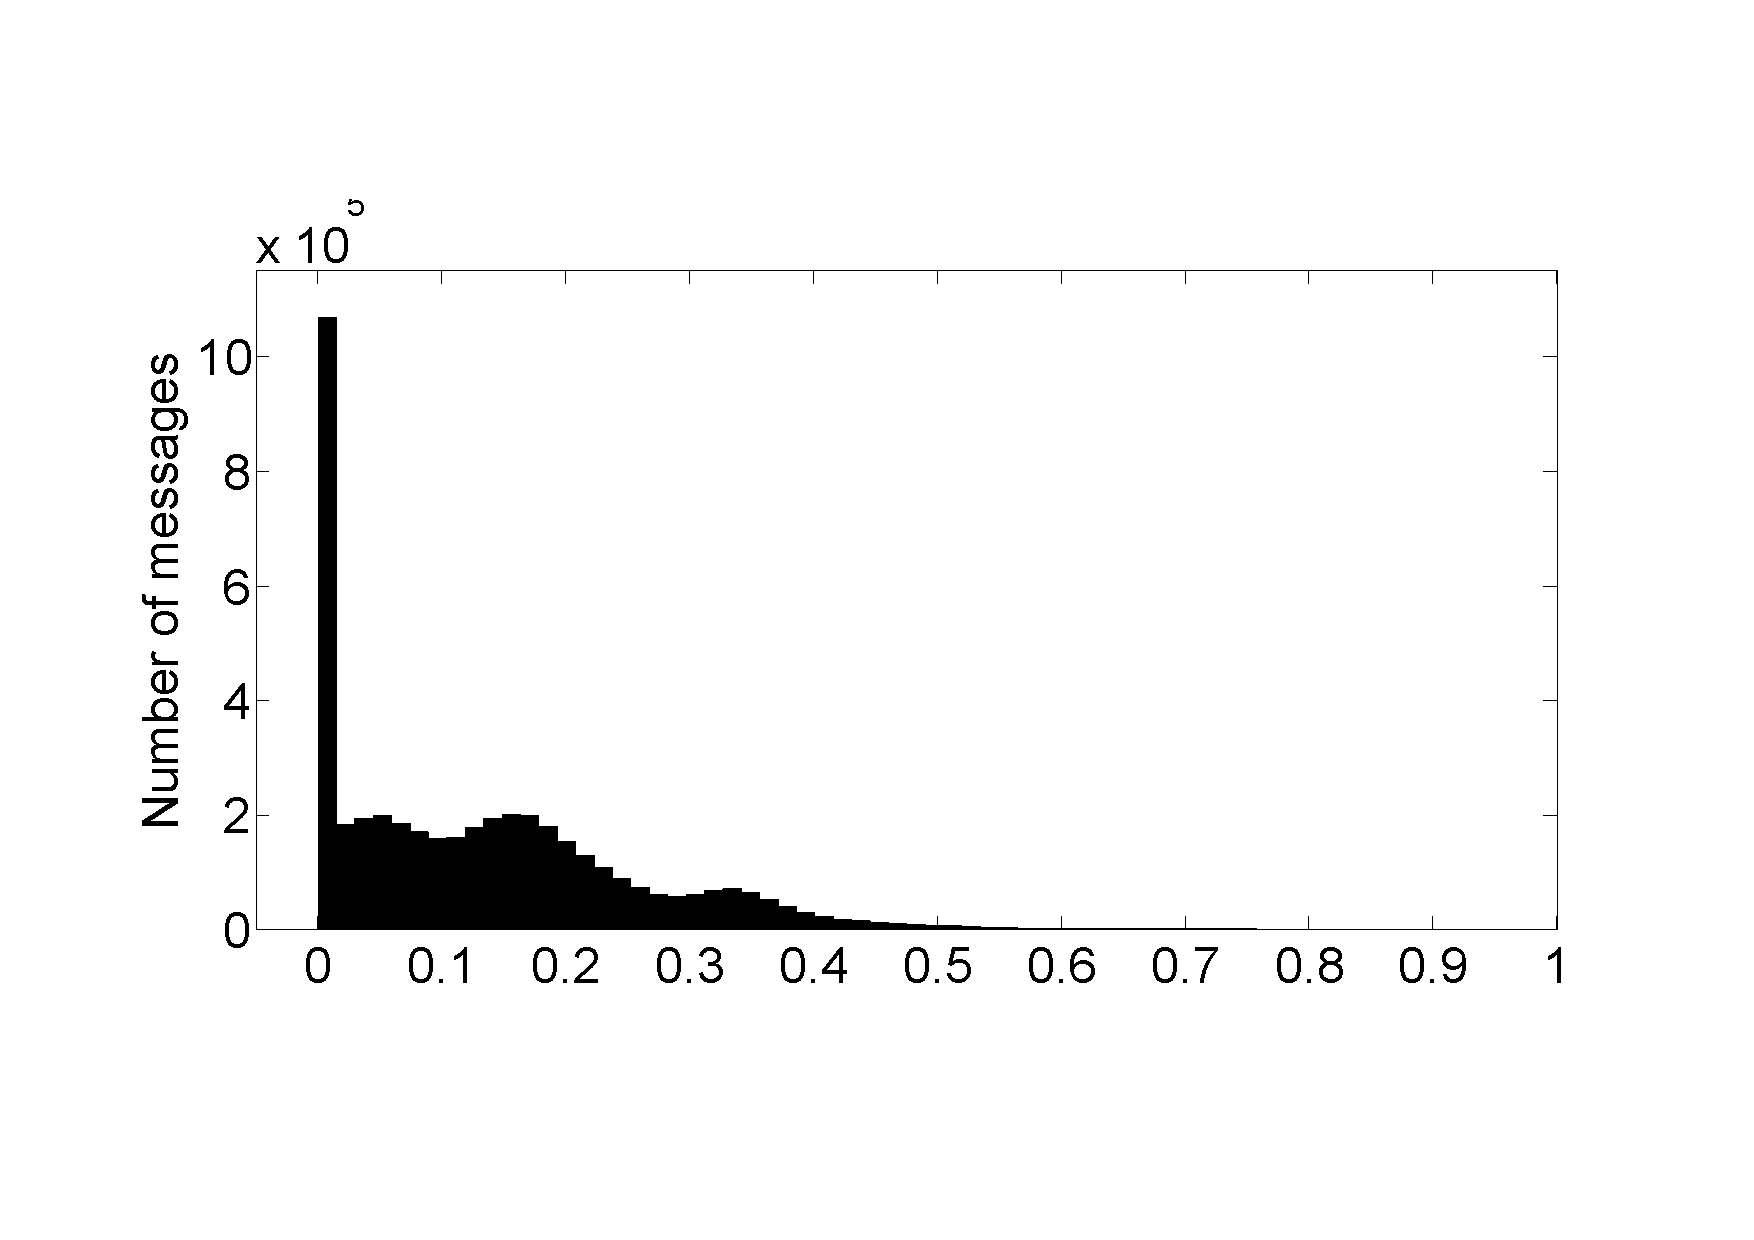
\includegraphics[clip=true, viewport=20mm 30mm 265mm 180mm, width=\columnwidth]{overall_get_ff}
 \caption{Overall retrieval responsiveness for fast retrieval}
 \label{fig_overall_get_ff}
\end{figure}
%
Figure \ref{fig_overall_get_ff} shows overall retrieval responsiveness for fast retrieval. The shape is similar to that of fast group retrieval in Figure \ref{fig_group_get_sf}, because in this case, fast retrieval returns the first result received. Since fast group retrieval is mostly faster then overlay retrieval, the overall retrieval distribution will closely match that of fast group retrieval.

\subsubsection{Parallel retrieval}
\begin{figure}[htbp]
 \centering
 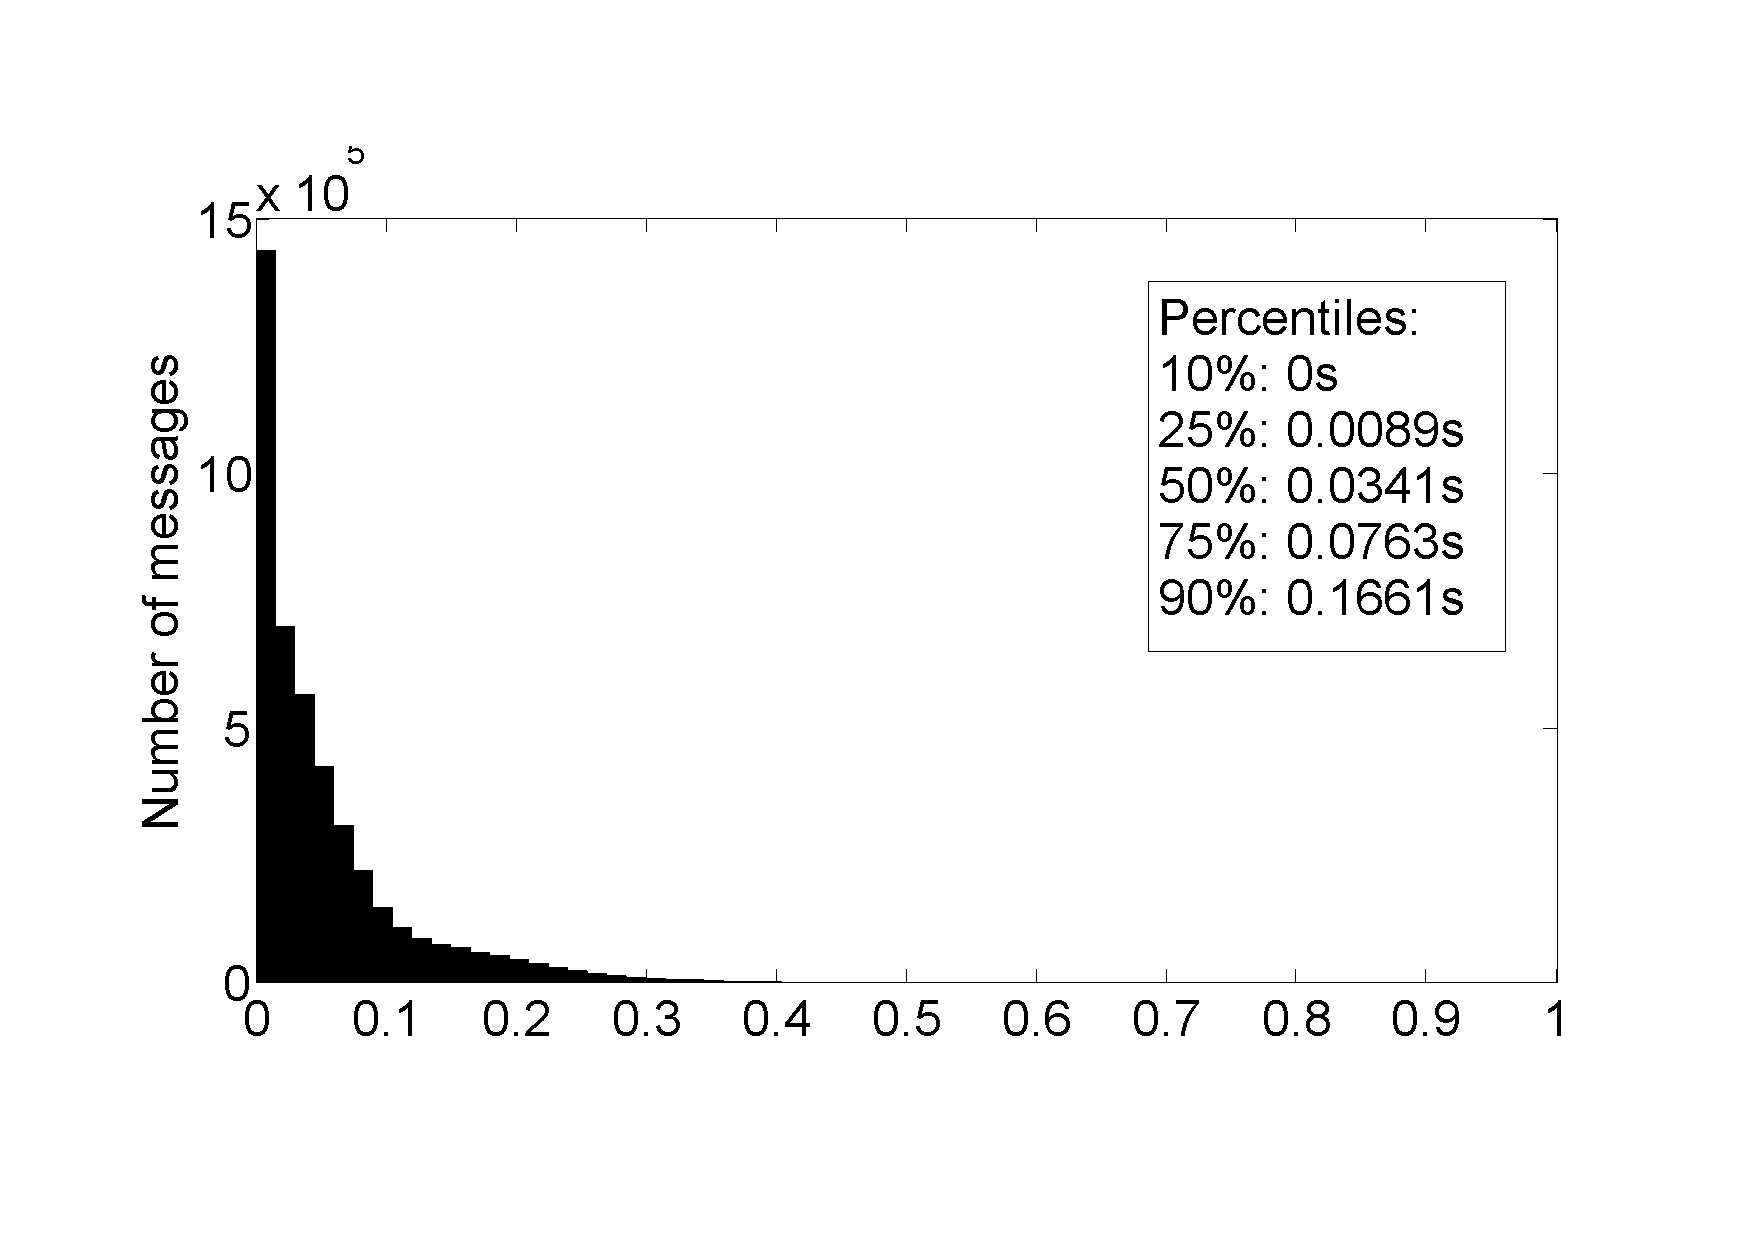
\includegraphics[clip=true, viewport=20mm 30mm 265mm 180mm, width=\columnwidth]{overall_get_fp}
 \caption{Overall retrieval responsiveness for parallel retrieval}
 \label{fig_overall_get_fp}
\end{figure}
%
Figure \ref{fig_overall_get_fp} shows the overall retrieval responsiveness for parallel retrieval. Overall parallel retrieval mirrors parallel group retrieval, since parallel retrieval is faster than overlay retrieval.

\subsection{Conclusion}

In this section some responsiveness distributions were shown. The first reason is that a fair comparison does not only consider the mean, but compares the distributions. These include the distributions for overlay storage and retrieval, fast and safe group storage, fast and parallel group retrieval, LAN performance, fast and safe overall storage, and fast and parallel overall retrieval. Secondly, it enables the highlighting of various structures and characteristics of storage and retrieval as they relate to certain quantities or mechanisms in Pithos. Thirdly, the distributions verify that Pithos meets the responsiveness and reliability design requirements.
 
When comparing the overall Pithos performance to the underlying group and overlay performance, it shows that Pithos is indeed a hybrid of those two storage types, but also that it is selecting the best qualities of both. This means that Pithos should perform better than the overlay chosen for use in Pithos.

\section{Performance for various group probabilities}
\label{group_probability_results}

The design of Pithos makes use of user groups and distance-based storage on a group layer, as stated in Sections \ref{grouping_design} and \ref{distance_based_design}. To verify the actual reliability and responsiveness of Pithos, it is necessary to investigate Pithos's performance for various group probabilities. In the final P2P MMVE architecture it is assumed that the percentage of in-group requests will be much higher than that of out-of-group requests, since distance-based storage is used. This assumption is based on the fact that with group-based distance-based storage, the objects that are frequently of interest to the user will be stored in that user's group.

\subsection{Experimental setup}

Because the exact probability that an object request will be for a group object is not yet known, a sweep is done for various group probabilities (the probability that a request is for a in-group object) to investigate the effect of group probability on Pithos's performance.

Because we expect that as the group probability changes, we will have a linear combination of group performance and overlay performance, the low overlay configuration is selected to better visualise this relationship.

The simplest storage and retrieval methods: fast storage and fast retrieval are selected. The specific type of group storage retrieval method is not important for this experiment, since the purpose of the experiment is to show the interplay between group and overlay storage.

As with the previous experiments, the following configuration parameters are chosen for reasons already discussed:
%
\begin{itemize}
\item Network of 2500 peers and 100 super peers.
\item Simulation length of 10,000s.
\item Using the Oversim SimpleUnderlayNetwork for the physical network.
\item Exponential object lifetime with 1800s mean and 300s TTL.
\item Object sizes of 1024 bytes.
\item Generating a store and retrieve request once every 5s.
\item Using Chord as overlay.
\item Storing six object replicas.
\end{itemize}

\subsection{Reliability}

\begin{figure}[htbp]
 \centering
 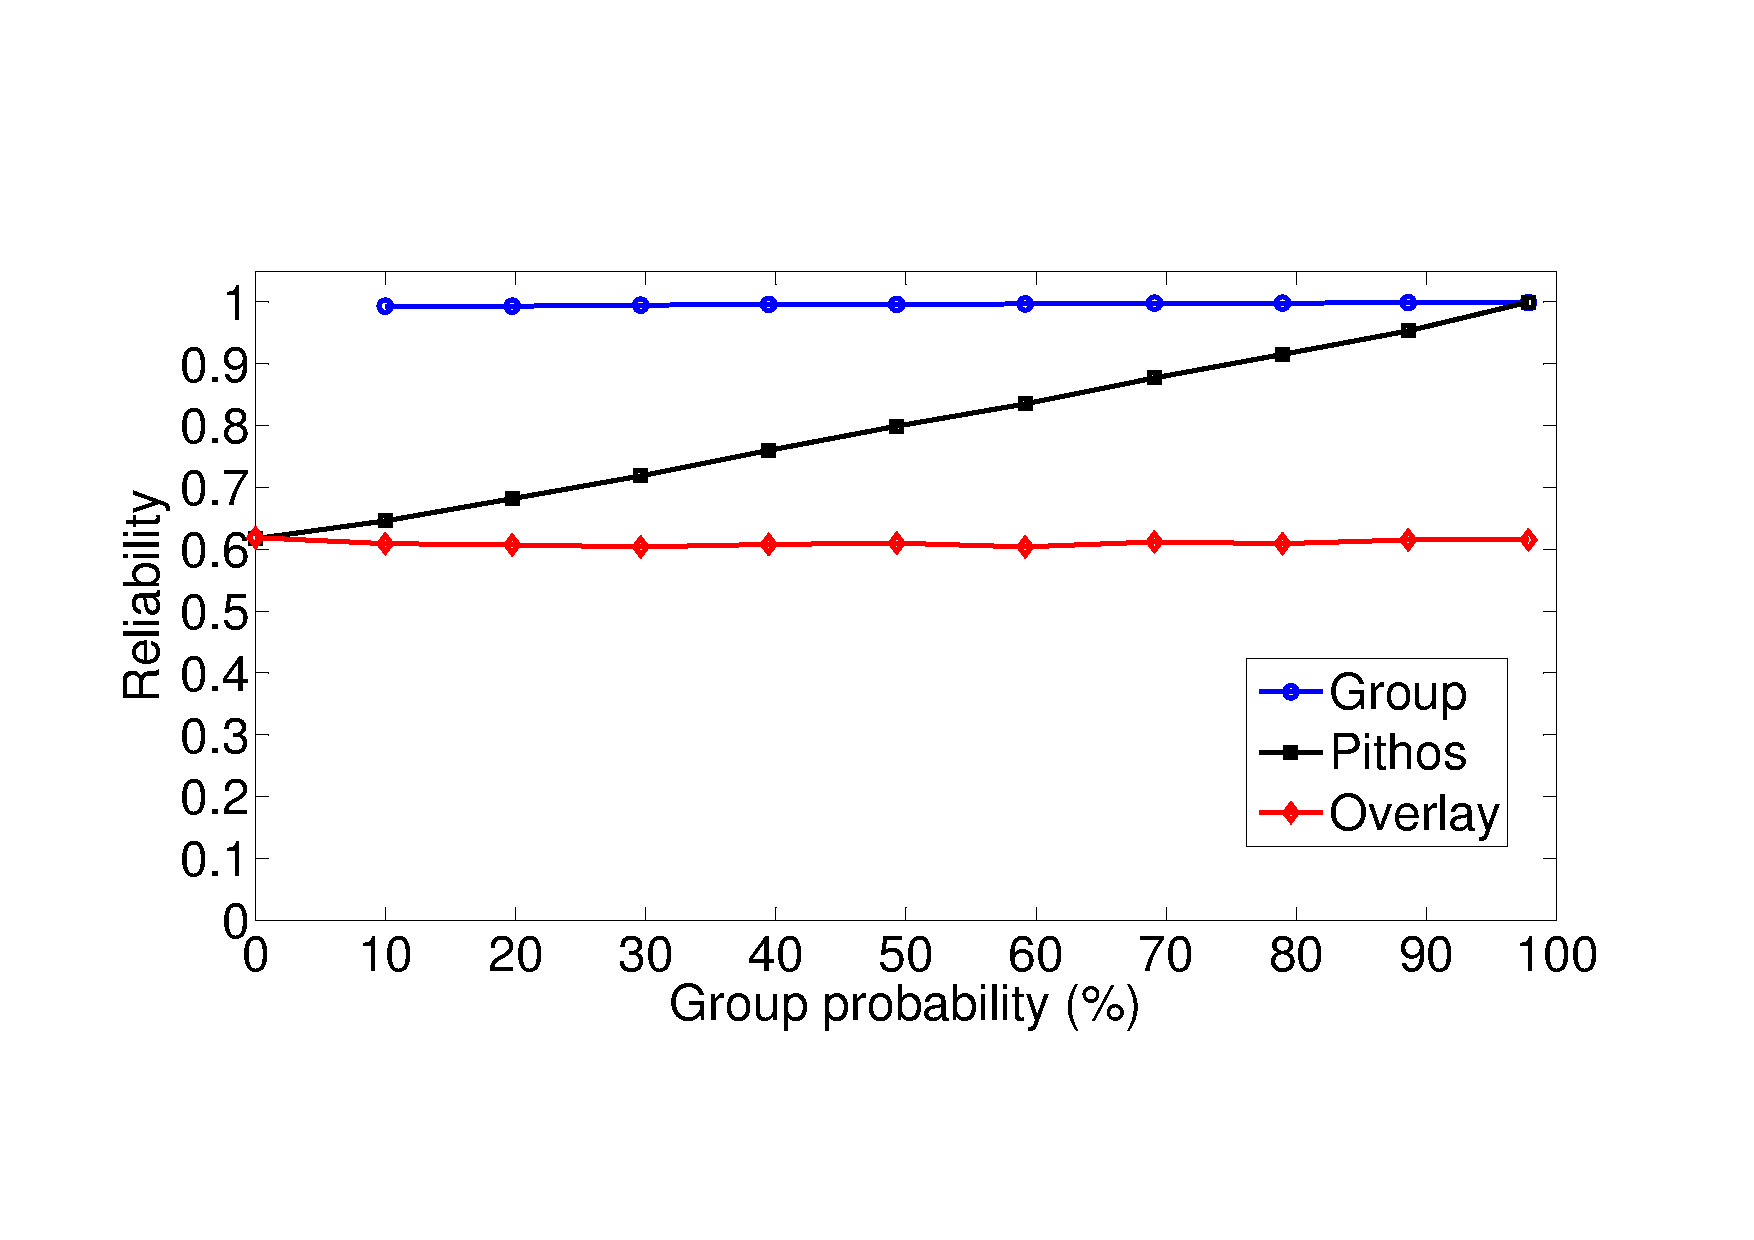
\includegraphics[clip=true, viewport=20mm 30mm 265mm 180mm, width=\columnwidth]{group_prob_rel}
 \caption{Reliability of Pithos, group storage and overlay storage for various group probabilities.}
 \label{fig_group_prob_rel}
\end{figure}
%
Figure \ref{fig_group_prob_rel} shows the effect group probability has on Pithos's overall reliability, compared with the underlying group storage and overlay storage reliabilities. The figure shows that the most reliable storage mechanism is group storage. It shows that group and overlay reliability are independent of the group percentage, which is as expected since the group storage and overlay storage modules are independent. Each request that is received from the higher layer (PithosTestApp) is relayed to both the DHT storage and group storage modules by the peer logic module.

When an object request is sent to group storage for an object that is not stored in that group, the group storage module reports that there does not exist such an object in the group and the request is not handled. The only possible reply is then from the overly storage module. Figure \ref{fig_group_prob_rel} shows that the overall Pithos reliability is a linear combination of group storage and overlay storage, weighted by the group probability.

These results can be verified theoretically by seeing that the reliability of Pithos is the union of the reliability of both group and overlay storage and is given by
%
\begin{align}
     \Gamma_{\textrm{Pithos}}& = \Gamma_{\textrm{group}} \cup \Gamma_{\textrm{overlay}} \\
     \textrm{which }
  E[\Gamma_{\textrm{Pithos}}]& = E[\Gamma_{\textrm{group}} \cup \Gamma_{\textrm{overlay}}] \notag \\
                             & = E[\Gamma_{\textrm{group}}] + E[\Gamma_{\textrm{overlay}}] \notag \\
                             & = P(\textrm{group})\Gamma_{\textrm{group}} + (1-P(\textrm{group}))\Gamma_{\textrm{overlay}}
\end{align}
%
where $\Gamma_{\textrm{Pithos}}$ is the overall Pithos reliability, $\Gamma_{\textrm{group}}$ is the group reliability, $\Gamma_{\textrm{overlay}}$ is the overlay reliability, and $P_{\textrm{group}}$ is the group probability.

This result shows that the reliability of Pithos varies linearly between overlay and group storage reliability as the group probability is varied. It should be noted that if a more reliable overlay was used, the medium or high configurations for example, the difference between group and overlay reliability is less. The low overlay configuration was just selected to better illustrate the linear relationship.

\subsection{Responsiveness}

\begin{figure}[htbp]
 \centering
 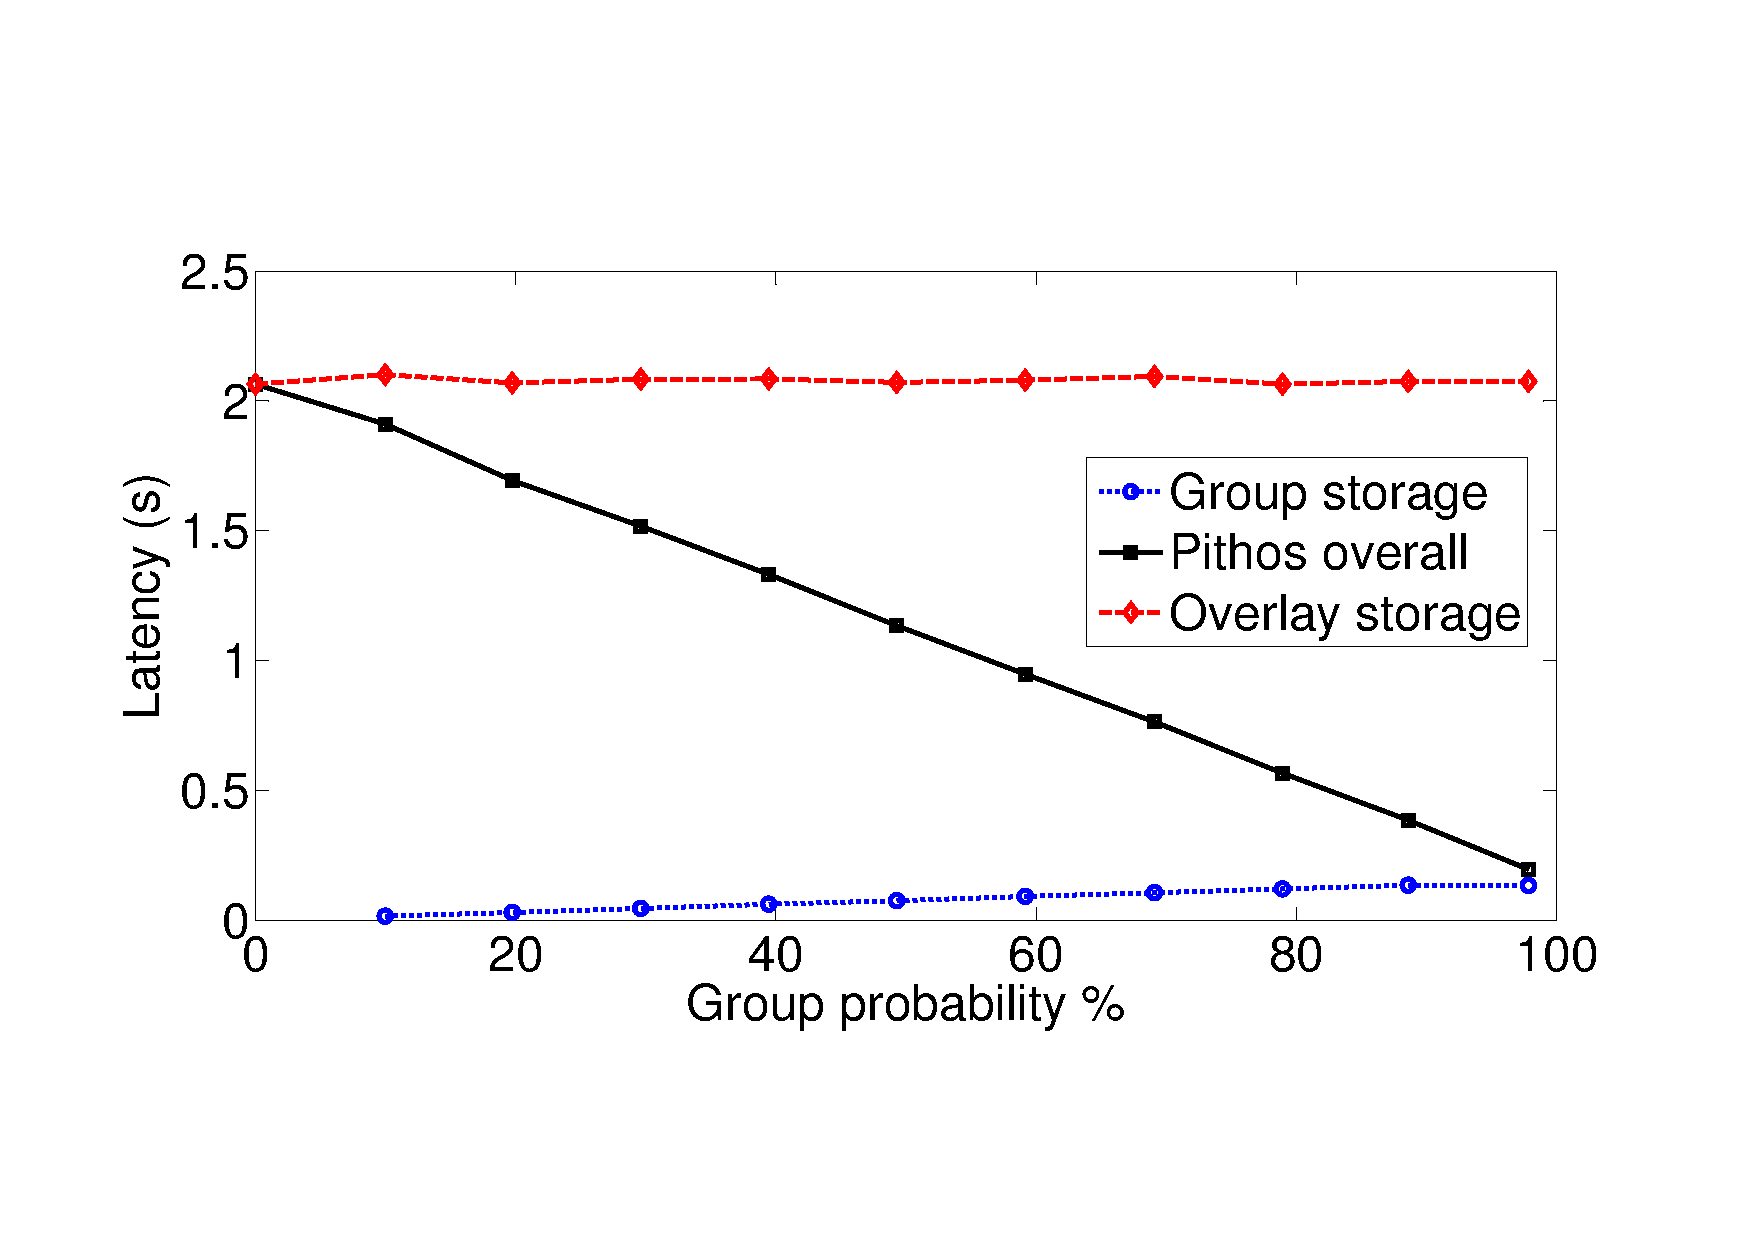
\includegraphics[clip=true, viewport=20mm 30mm 275mm 180mm, width=\columnwidth]{group_prob_resp}
 \caption{Responsiveness of Pithos, group storage and overlay storage for various group probabilities.}
 \label{fig_group_prob_resp}
\end{figure}
%
Figure \ref{fig_group_prob_resp} shows the responsiveness of Pithos compared with the underlying responsiveness of group and overlay storage. Take note that a lower value is preferred in this graph and that low latency is high responsiveness. As with the reliability, overall responsiveness is also shown to be a linear combination of group and overlay responsiveness.

An apparent anomaly is the group storage latency that increases with an increase in group probability. Recall that if a request is sent to group storage for an object not in the group, group storage immediately returns failure. The failure response is recorded as a response from group storage, even if this response is a failure.

The lower the group probability, the more failure responses are returned by group storage, which are returned instantly. It is these responses that decrease the mean group storage latency for lower group probabilities. When failure responses are ignored, group latency remains constant at the value of 100\% group probability.

\subsection{Bandwidth}
\label{group_probability_bandwidth}

\begin{figure}[htbp]
 \centering
 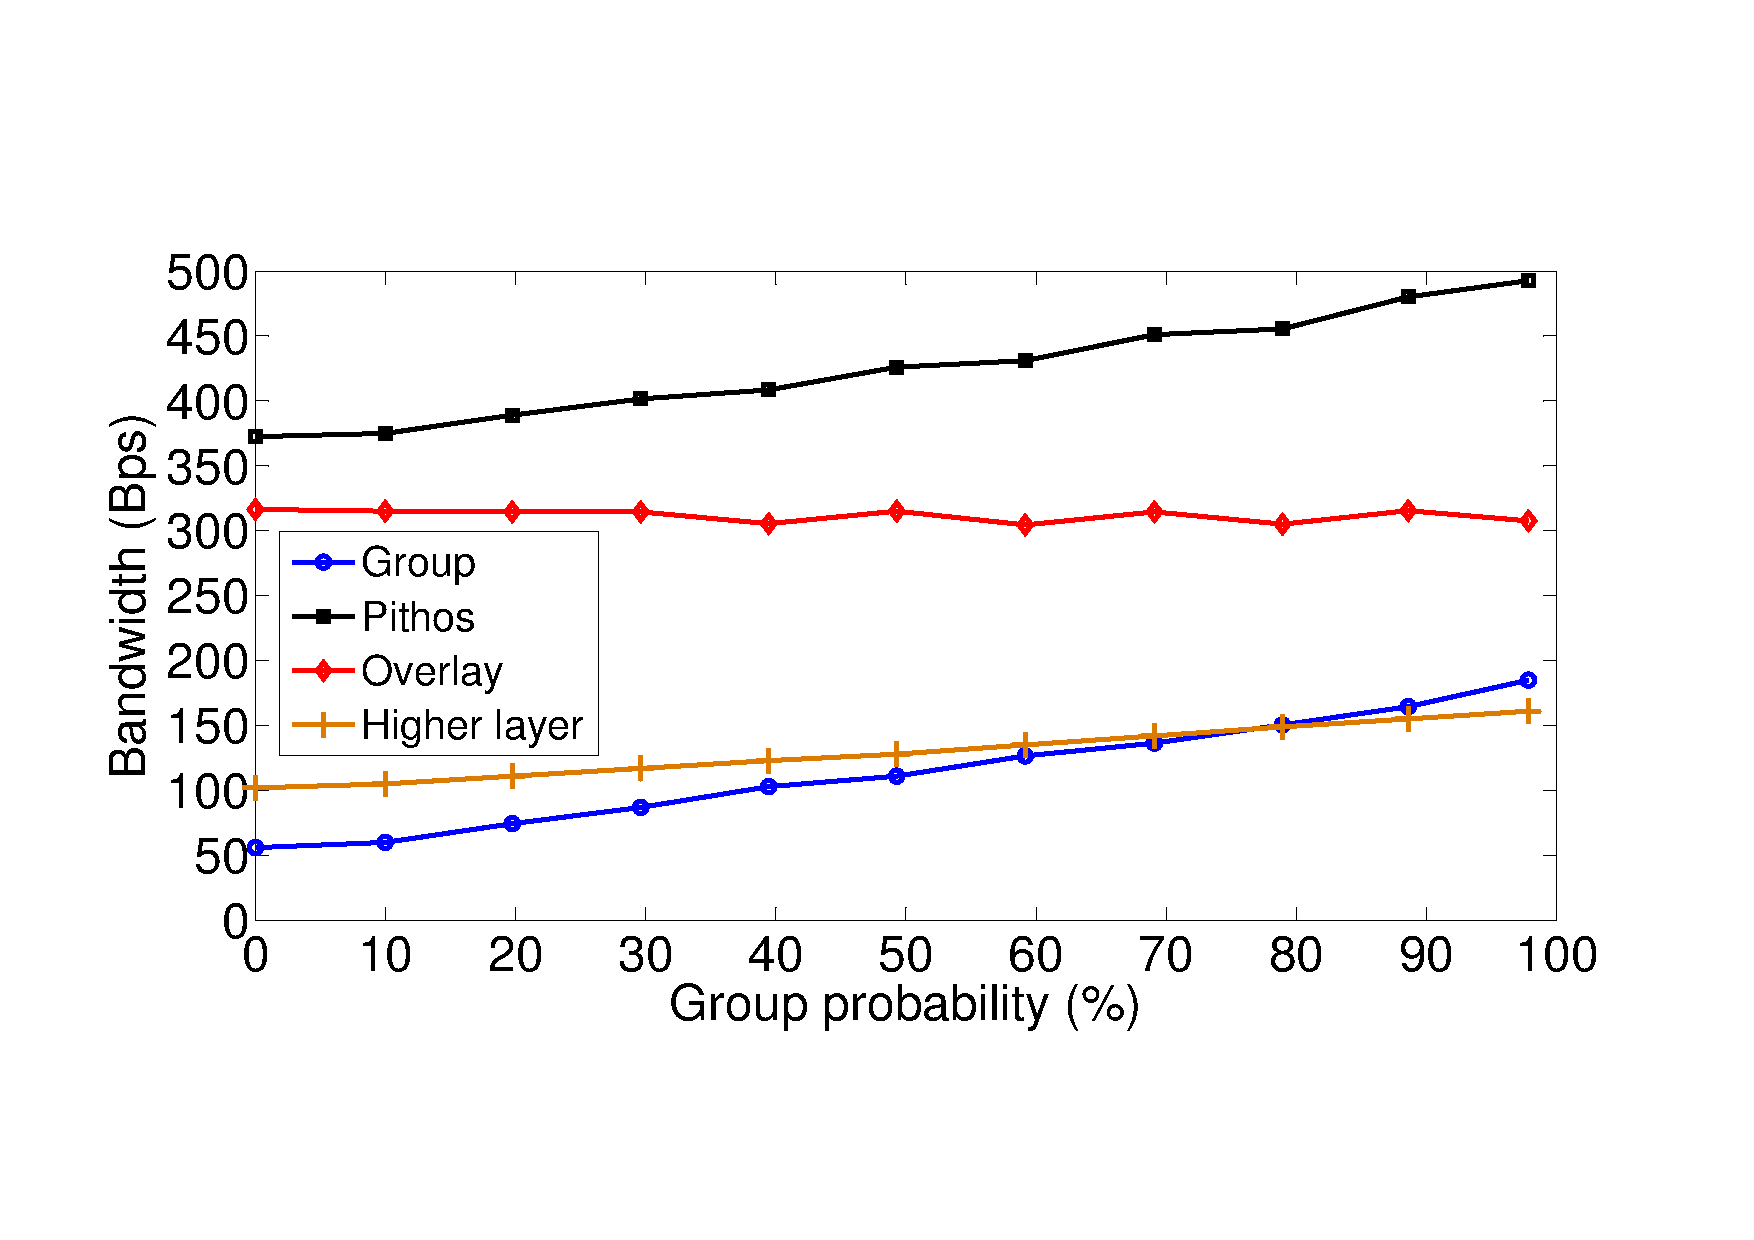
\includegraphics[clip=true, viewport=15mm 30mm 270mm 180mm, width=\columnwidth]{group_prob_bw}
 \caption{Bandwidth usage of Pithos, group storage and overlay storage for various group probabilities, as well as the bandwidth sent to, and received from Pithos.}
 \label{fig_group_prob_bw}
\end{figure}
%
Figure \ref{fig_group_prob_bw} shows the bandwidth requirements of Pithos in bytes per second (Bps). Pithos, group and overlay bandwidths show the mean of the inbound and outbound bandwidth. Figure \ref{fig_group_prob_bw} also shows the underlying bandwidth requirements of group storage and overlay storage. To determine the actual overhead that Pithos requires, the graph also shows the amount of data that is sent to, and received from, Pithos, from and to the higher layer (PithosTestApp).

Figure \ref{fig_group_prob_bw} shows that overlay storage bandwidth remains constant, but that group storage bandwidth increases. Overlay storage remains constant, because no matter what the group probability is, the overlay storage is always queried for a data item and a data item is returned with the same probability (based on the reliability). Group storage, on the other hand, only returns data if the object exists within the group. Higher group probability means that more objects are requested from within the group, which means that group probability will return more objects and thereby use more data.

As shown, the overall Pithos bandwidth the the sum of the bandwidth required by group and overlay storage.

The data sent to Pithos is less than the data received from Pithos, because more retrieval requests are performed in the simulation than storage requests.

The graph shows that the Pithos overhead is approximately 76\% of data in the network, where, depending on the group probability, 85\% to 62\% of overhead is contributed by overlay storage for the low overlay configuration.

\subsection{Conclusion}

This section reviews the performance of Pithos for various group probabilities and also shows the interaction between overlay and group storage in terms of reliability, responsiveness and bandwidth.

All the experiments verified that for a low group probability, the characteristics of overlay storage are dominant and for high group probability, the characteristics of group storage are dominant. As previously stated, because of the distance-based storage design, high group probabilities are expected.

What was shown in this section is that overlay storage provides lower reliability than group storage with relatively high bandwidth requirements, compared to group storage. This underpins the need for an overlay better suited to environments with network churn and improved lookup reliability. Before overlay efficiency can be improved, it is therefore important to create a grouping algorithm that has the highest possible group probability.

\section{Security}
\label{malicious_results}

In this section we verify that Pithos meets the security design requirements specifically, we investigate the object retrieval reliability in the presence of malicious users in the P2P network.

As a result of its design, fast retrieval is not resistant to malicious users, since it will retrieve corrupted objects, if the first retrieval response was received from a malicious user. Safe retrieval uses a quorum mechanism to respond with the object, which the majority of queried peers agree is correct. We therefore expect safe retrieval to be resistant to the presence of malicious users.

We also wish to investigate the reliability of the security mechanism as a function of the number of queried peers. We expect the reliability to increase with a larger quorum, but at the expense of a slower response time and an increase in bandwidth.

\subsection{Experimental setup}

Each object in Pithos has a double value attribute that is set to a random value when an object is created for the simulation. The value of the object is stored in PithosTestApps's global object list. It should be noted that for simulation purposes, an object's size is not related to its content. An object's size is set using a random distribution and this is the value used to compute transmission bandwidth and latency.

Whenever a malicious node receives a retrieval request it replies with a modified version of the requested object. The object is modified by modifying the object value. An object is assigned a uniformly random value by a malicious node. Because of the way objects are altered, we implicitly assume that there exists no collusion in the network. When PithosTestApp receives a requested object, it checks that object against the global object list to determine whether the correct object was received. PithosTestApp then records Pithos's reliability.

Pithos selects the object that is the same in a majority of responses and sends it to the higher layer. If no object has a majority, a failure response is sent to the higher layer.

The percentage of users that are malicious is varied from 0.0 to 1.0 in steps of 0.125. A comparison of safe retrieval is performed by first retrieving four of the six stored replicas and then increasing the number of retrievals to six.

As with the previous experiments, the following configuration parameters are chosen for reasons already discussed:
%
\begin{itemize}
\item Fast group storage is used.
\item Network of 2500 peers and 100 super peers.
\item Simulation length of 10,000s.
\item Using the Oversim SimpleUnderlayNetwork for the physical network.
\item Exponential object lifetime with 1800s mean and 300s TTL.
\item Object sizes of 1024 bytes.
\item Generating a store and retrieve request once every 5s.
\item Using Chord as overlay.
\item Storing six object replicas.
\item All requests are for local group objects.
\end{itemize}

\subsection{Results}
\begin{figure}[htbp]
 \centering
 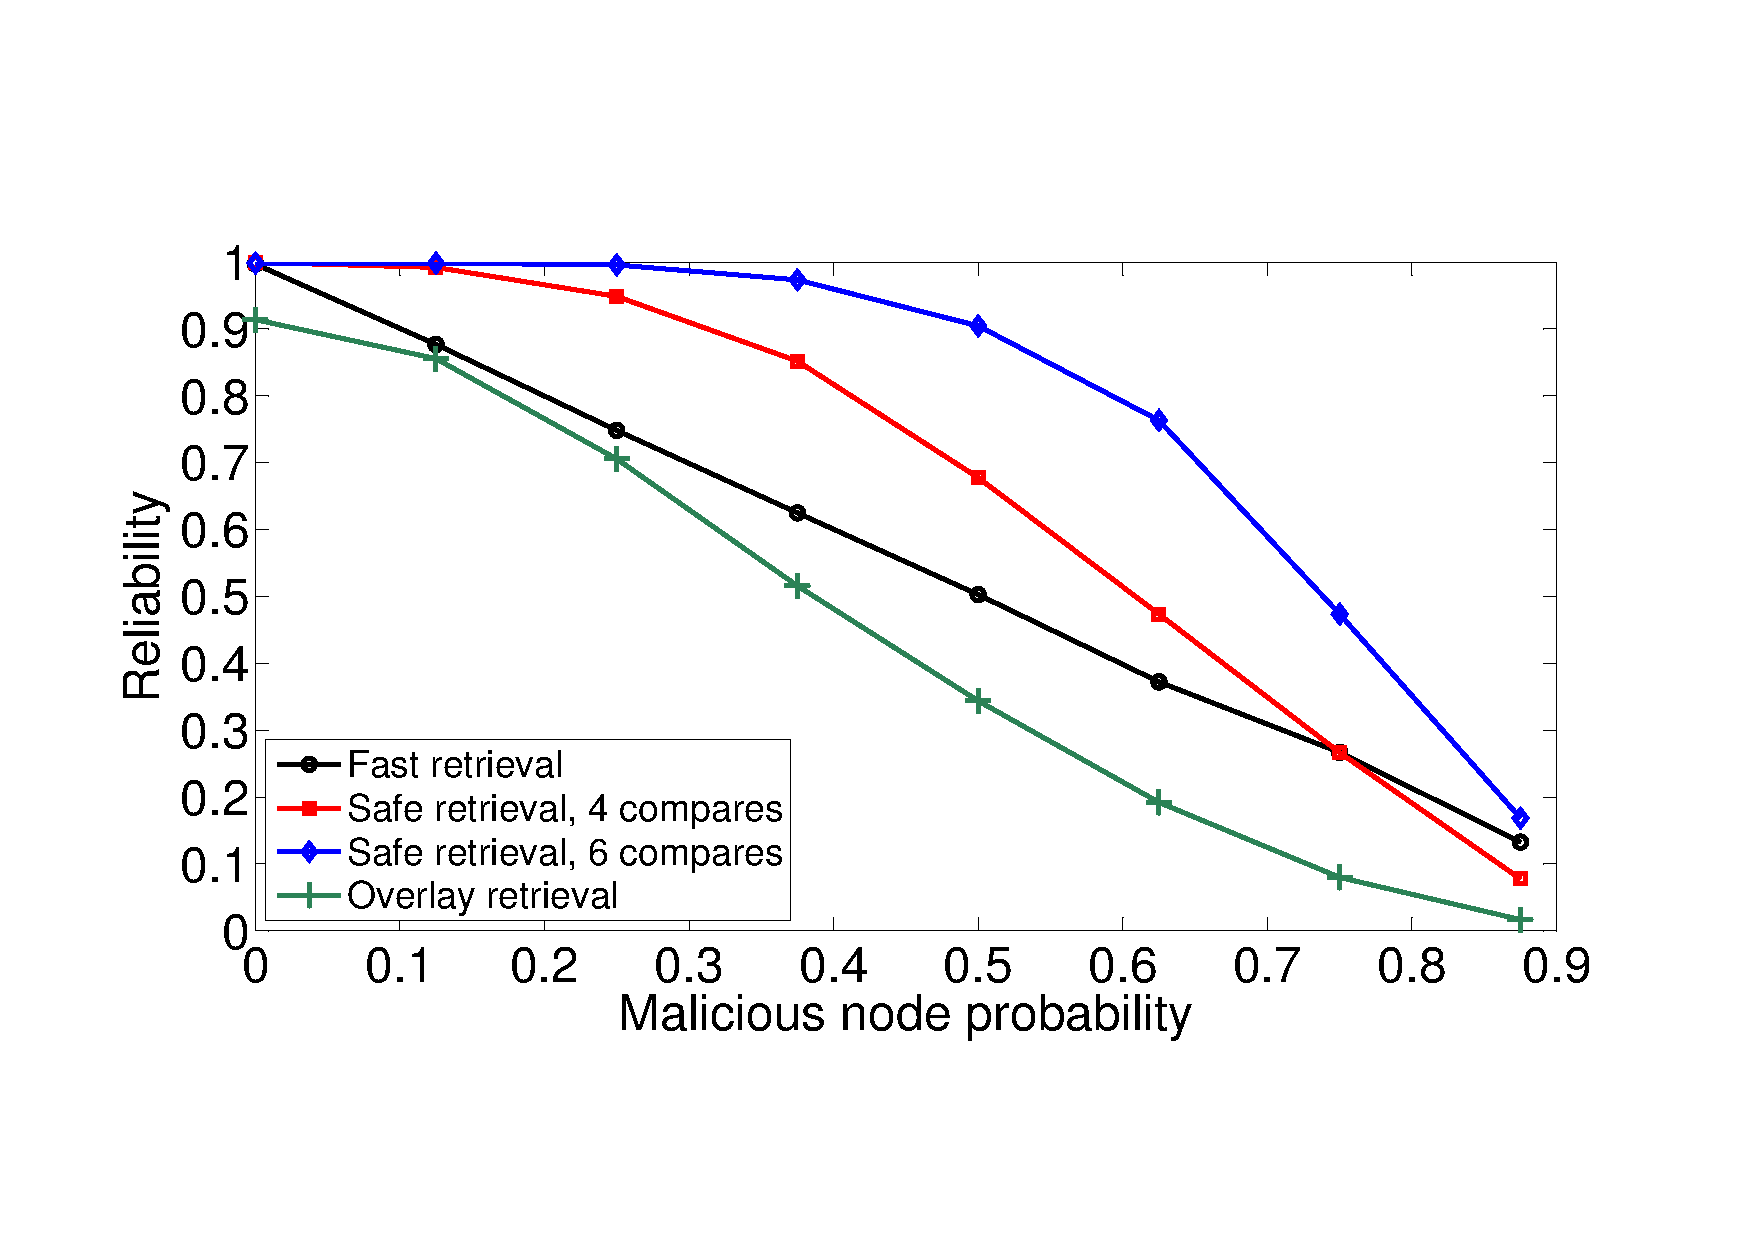
\includegraphics[clip=true, viewport=20mm 30mm 270mm 175mm, width=\columnwidth]{malicious_nodes_rel}
 \caption{Reliability of various Pithos retrieval schemes for varying factors of malicious node probability.}
 \label{fig_malicious_nodes_rel}
\end{figure}
%
Figure \ref{fig_malicious_nodes_rel} shows Pithos's reliability as a function of the percentage of malicious users in the network for both the fast retrieval and safe retrieval schemes. The fast retrieval reliability is almost the same as the malicious user percentage. System reliability for fast retrieval is the product of the malicious user factor and the system reliability under no malicious users.

The reason for this direct relationship is because the probability of an object retrieval being corrupted in the network is equal to the probability of a peer being malicious, since a malicious peer corrupts all objects returned and a non-malicious peer corrupts none of the objects returned. The overall probability is then the probability that an object retrieval would have succeeded if no malicious nodes were present, multiplied by the probability of nodes being malicious.

Figure \ref{fig_malicious_nodes_rel} also shows the improvement received from using safe retrieval. The curve shows that safe retrieval provides greater benefit for smaller factors of malicious nodes. As soon as the majority of objects are corrupted, object reliability drops significantly.

The figure also shows improved reliability, when more received objects are compared to select a majority. Retrieving more objects for comparison will, however, increase bandwidth requirements. Bandwidth increases in line with that shown in Section \ref{bandwidth_requirements}, because safe retrieval is parallel retrieval, but for an additional compare operation. It should be noted that more retrievals than compares may be performed to increase responsiveness at the cost of additional bandwidth.

An interesting situation arises, where safe retrieval reliability drops below fast retrieval reliability. When a majority can no longer be identified by safe retrieval, a failure response is sent up. This is as opposed to fast retrieval that sends any object received. It is possible the the object that was selected by fast storage was not maliciously altered, but also not in the majority. In this scenario, fast retrieval will sometimes send objects to the higher layer that were correct, where safe storage just responded with failure, because it couldn't be sure. Because in practice, the higher layer will not know whether an object is corrupted or not, it seemed more prudent to only send objects to the higher layer where Pithos was reasonably sure the object was unaltered.

Figure \ref{fig_malicious_nodes_rel} also shows the performance of overlay storage under the presence of malicious nodes if no security mechanisms are implemented in overlay storage. The performance degrades as the percentage of malicious users increase. The performance is also worse than the overall Pithos performance.  It should be noted that the overall Pithos performance is not influenced by Overlay storage in this graph, since 100\% group probability is used. For lower percentages of group probability, the linear relationship between group and overlay storage, explored in Section \ref{group_probability_results} exists.

\subsection{Conclusion}

The section shows that Pithos's safe retrieval mechanism can be used to increase reliability under malicious users at the cost of responsiveness and bandwidth. With malicious users usually present in a virtual world, this cost is always acceptable. During the lifetime of the virtual world, it is important to monitor that malicious user percentage, to determine how parameters, such as number of retrieve requests and number of compares, should be adjusted to combat the threat while minimising bandwidth and maximising responsiveness.

In practice, a low malicious node factor is expected, since it is assumed that cheaters are in the minority. If the virtual world has a majority of cheaters, it will most likely not be sustainable.

\section{Object distribution (fairness)}

One of the key reasons objects are distributed amongst groups is to achieve storage fairness. As described in Section \ref{fairness_requirement}, fairness is required to ensure that all peers contribute equally to the P2P network.

\begin{figure}[htbp]
 \centering
 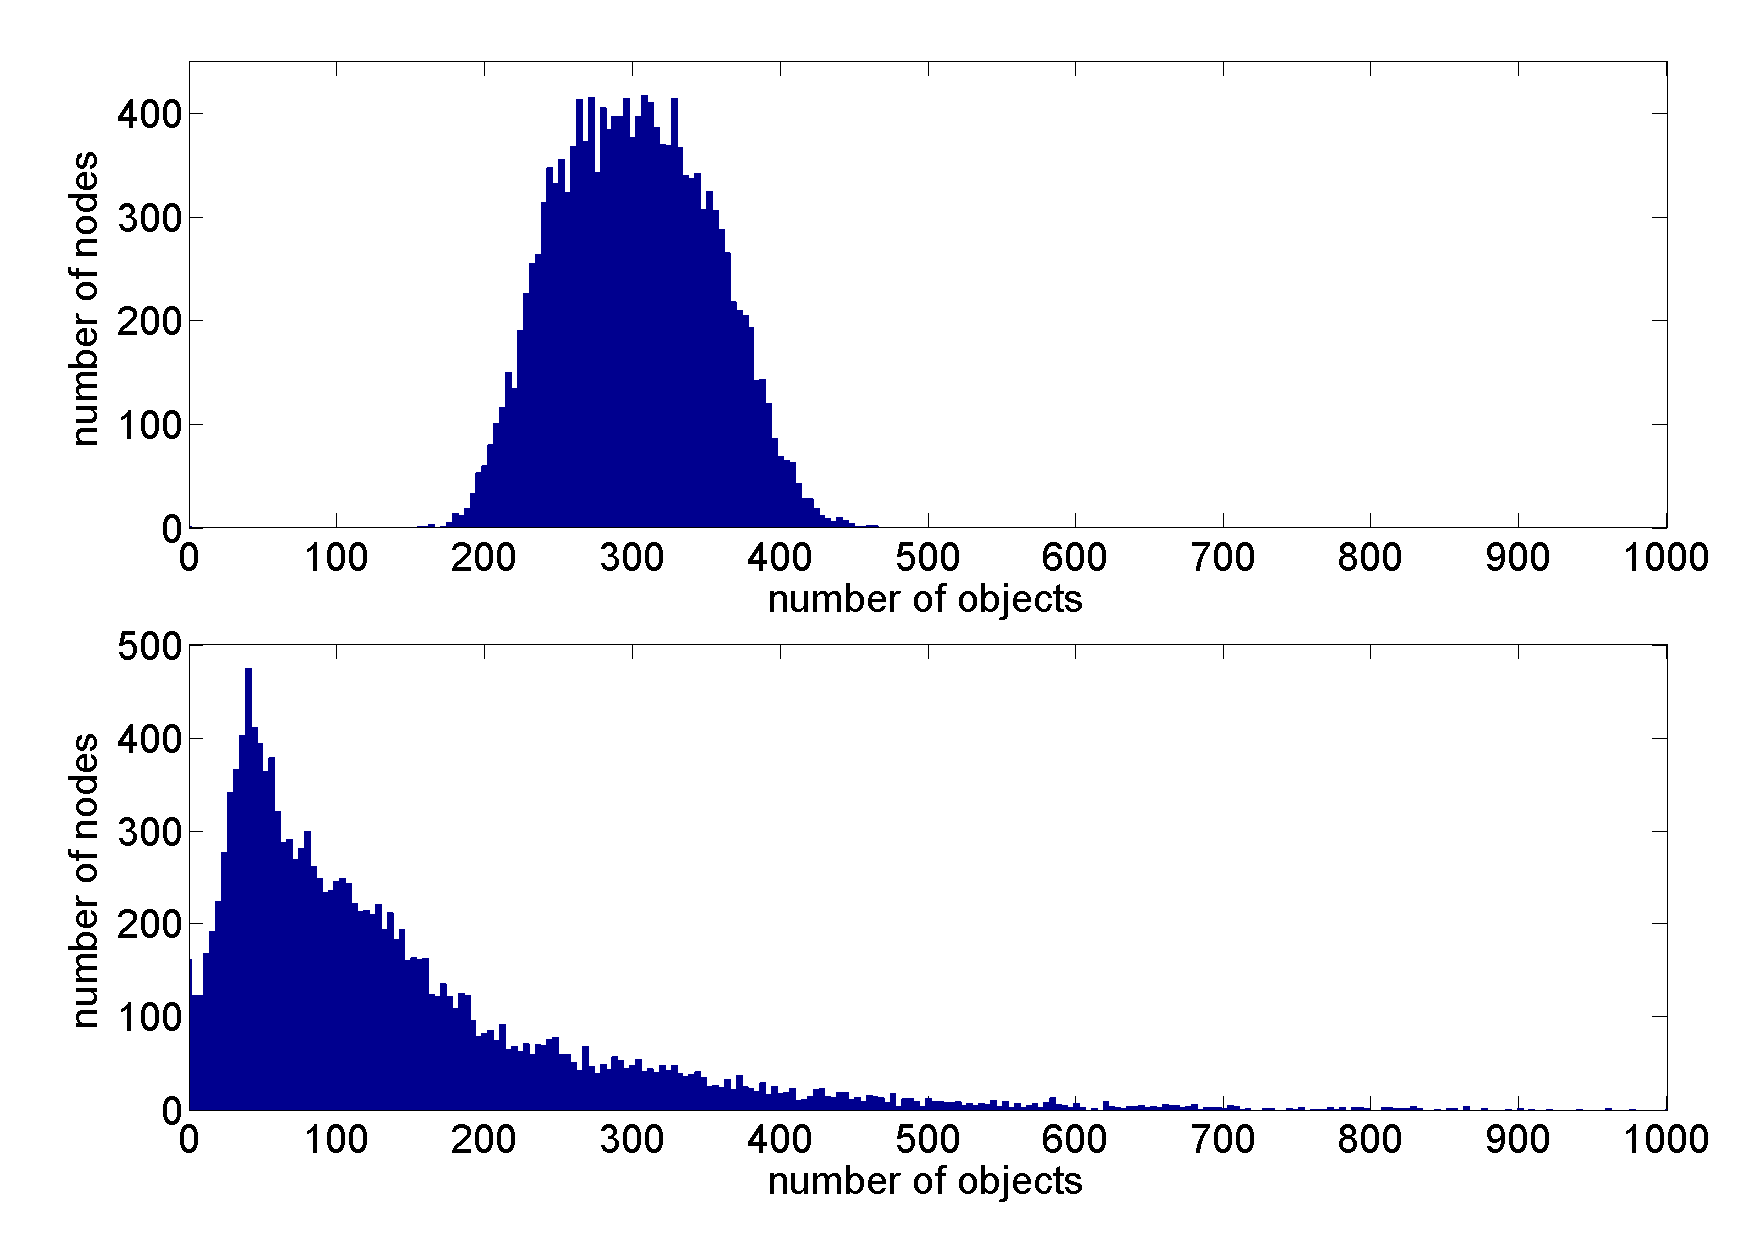
\includegraphics[clip=true, viewport=1cm 0.5cm 28.5cm 20cm, width=\columnwidth]{RootRepOverlayObjects}
 \caption{Top: Distribution showing the number of peers that store a certain number of group objects. Bottom: Distribution showing the number of peers that store a certain number of overlay objects.}
 \label{fig_group_overlay_objects}
\end{figure}
%
To evaluate the fairness, we evaluate the standard deviation of the number of objects stored per peer. Figure \ref{fig_group_overlay_objects} (top) shows the distribution of group objects over nodes in the network. The figure shows how many nodes store how many objects. The distribution has a mean and standard deviation of 302 and 51 objects per node respectively.

Figure \ref{fig_group_overlay_objects} (bottom) shows the distribution of overlay objects in Pithos with a mean and standard deviation of 153 and 189 objects per node respectively. Comparing the standard deviations of group storage to overlay storage, it appears that group storage is fairer than overlay storage.

\begin{figure}[htbp]
 \centering
 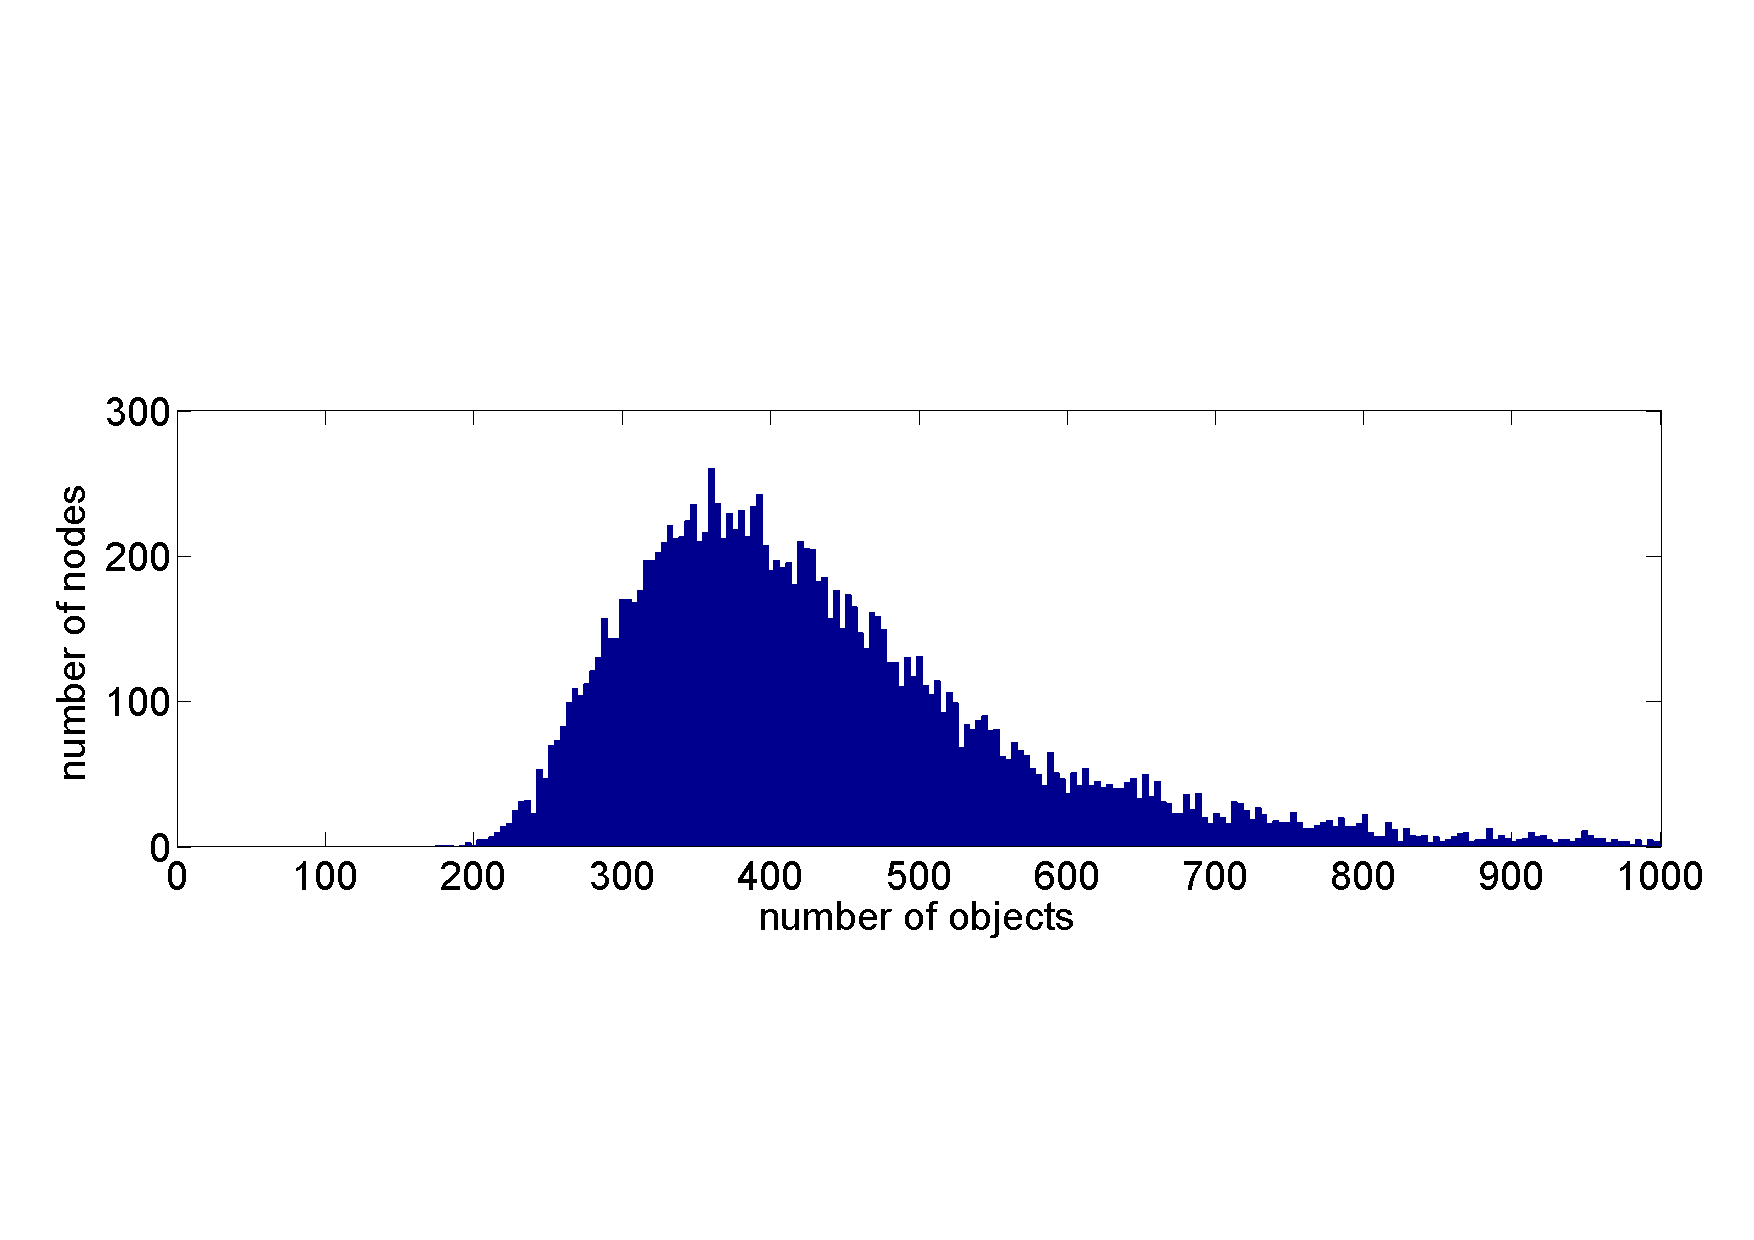
\includegraphics[clip=true, viewport=1cm 5cm 29cm 14.5cm, width=\columnwidth]{Objects}
 \caption{Combined object number distribution}
 \label{fig_objects}
\end{figure}
%
Figure \ref{fig_objects} shows the combined object distribution of Pithos, with a mean and standard deviation of 453 and 200 objects per node respectively. This shows that the fairness of Pithos is currently dominated by the fairness of the overlay and that Pithos is as fair as overlay storage.

What should be concluded from this section is that there does no exist a minority of peers in Pithos that store the majority of the data. All peers are required to contribute to the P2P network.

\section{Performance under object repair}
\label{repair_results}

Object replicas inserted into Pithos will all eventually disappear due to network churn. The rate at which replicas are removed from the network can be reduced by employing object repair. This enables Pithos to trade storage space for network bandwidth, by using fewer replicas with a higher repair rate. Network bandwidth can also be saved by having more replicas and a lower repair rate.

The effect of node replicas on the reliability and bandwidth efficiency of Pithos will be explored in this section. Reliability is tightly coupled to the lifetime of nodes, since nodes that live longer will store objects longer, meaning objects stored on nodes with longer expected lifetimes will have longer expected lifetimes. The main reason for being unable to retrieve an object from Pithos is because a peer has left the network. It is, therefore, expected that if nodes life longer the system reliability increases.

\section{Scalability}

As identified in Section \ref{scalability_req}, a key requirement of P2P MMVEs is that they should be scalable. It was argued that scalability is achieved when all other requirements are met, for a large numbers of nodes. The results shown thus far have been for a \emph{sufficiently scalable} system of 2500 nodes.

To show the scalability of the Pithos design and implementation, Pithos is simulated for 10,000 peers and 400 super peer, four times more peers and super peers than previously simulated.

\subsection{Simulation setup}

The fast storage and fast retrieval setup was used, with the same configuration parameters as in Section \ref{store_retrieve_exp_setup}:
%
\begin{itemize}
\item Nodes lifetimes of 1800s,
\item 98.3\% group probability,
\item medium overlay configuration,
\item 300s object TTL and
\item no repair.
\end{itemize}


The 10,400 peer simulation setup was not shown during the previous sections, because of the resources required to complete it. The simulation requires 19 hours of run time and 14 GB of RAM on an Intel Core i7, 3 GHz, quad core processor. A simulation on this scale would not have been possible using anything other than Oversim's simple underlay. The efficiency of the C++ language also provides great gains in terms of both processer and memory efficiency.

Although lengthy, a 19 hour simulation time is still a feasible time to performs simulations in.

\subsection{Results}

For both cases, the data from the higher layer was still measured as 4 Bps sent to Pithos and 157 Bps received from Pithos.

\begin{table}[htbp]
\centering
\begin{tabular}{|c|c|c|c|c|}
\hline
Number of peers & Module & Reliability & Responsiveness (s)  & Bandwidth \\
\hline
2600            & Overall&  0.9970     &   0.192             & 1370/1380 \\
2600            & Group  &  0.9775     &   0.134             & 187/183   \\
2600            & Overlay&  0.9140     &   1.760             & 1183/1197 \\
10,400          & Overall&  0.9971     &   0.191             & 1647/1657 \\
10,400          & Group  &  0.9819     &   0.134             & 180/177   \\
10,400          & Overlay&  0.9006     &   1.960             & 1467/1480 \\
\hline
\end{tabular}
\caption{Responsiveness and reliability of fast and parallel retrieval for safe and fast storage.}
\label{tab_pithos_scalability_results}
\end{table}
%
Table \ref{tab_pithos_scalability_results} shows the scalability of Pithos for large numbers of peers. Comparing group storage, it is evident that the reliability and responsiveness of the 2600 peer case is the same as that of the 10,400 peer case. Also of note is that group storage requires no more bandwidth for larger numbers of nodes. The results show group storage to be very scalable.

Overlay storage, however, fares worse both in responsiveness as well as required bandwidth.

Overall, Pithos is as reliable and responsive for 2600 peers as it is for 10,400 peers, with the exception that it uses somewhat more bandwidth, which has been shown to be as a consequence of the overlay storage not scaling as well as group storage.

This section shows that Pithos is scalable for large numbers of nodes in terms of responsiveness, reliability as well as bandwidth requirements.

\subsection{Experimental setup}

\begin{itemize}
\item Node lifetimes are varied from 100s to 1800s in irregular steps that are closer together for lower peer lifetimes.

\item Fast group storage is used.

\item Fast group retrieval is used for the no repair, leaving repair and periodic repair cases.

\item Parallel retrieve with no repair is also compared.

\item Six object replicas are stored.

\item Object TTL is set to 1000s.
\end{itemize}

\subsection{Reliability}

\begin{figure}[htbp]
 \centering
 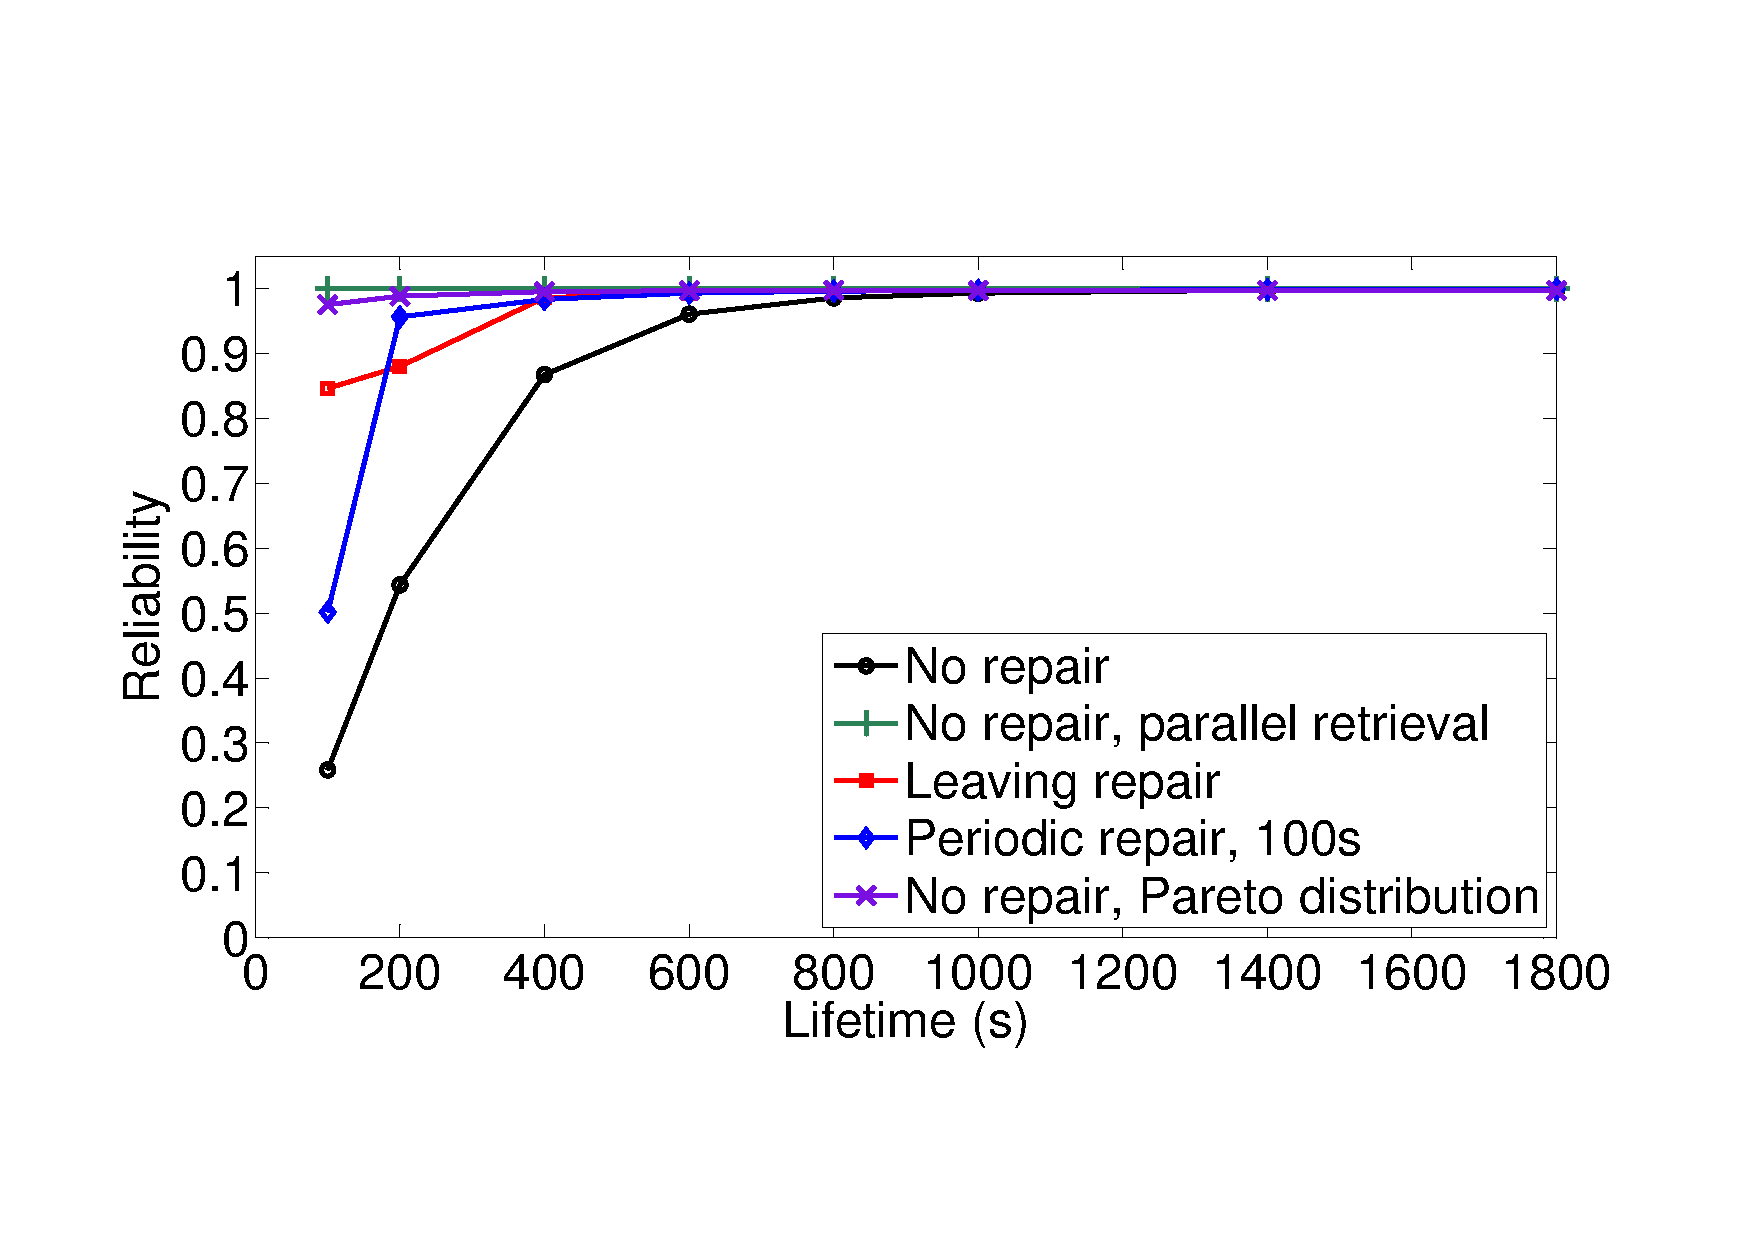
\includegraphics[clip=true, viewport=15mm 30mm 275mm 180mm, width=\columnwidth]{repair_rel}
 \caption{Reliability of Pithos for various node lifetimes, comparing no repair, no repair with parallel retrieval, leaving repair and periodic repair with 100s periods.}
 \label{fig_repair_rel}
\end{figure}
%
Figure \ref{fig_repair_rel} shows request reliability for various node lifetimes for no repair, no repair using parallel retrieve, leaving repair and periodic repair.

As expected, doing no repair does not cope well with short node lifetimes compared to an object TTL of 1000s. The object TTL is important when evaluating performance, since a network that requires objects to be stored for longer has to maintain the object replicas for a longer amount of time. When the expected node lifetime is equal to the object TTL at 1000s, the reliability of the system when not using repair is similar to the the system reliability when repair is used.

This observation is helpful when designing a P2P MMVE. Objects might be classified according to how long their should remain in the system. Objects that should only remain in the system for approximately the same amount of time as the expected user session time need not use repair mechanisms, if a sufficient number of replicas are used.

When node lifetimes are the same as the periodic repair interval, leaving repair copes better than periodic repair. The periodic repair mechanism might be adjusted to less than the minimum expected node lifetime in the system, but this will increase the load on the super peer, which has to perform the periodic checks. From the data is seems that leaving repair might be able to better handle a situation where node lifetimes have a high dynamic range, since the rate at which nodes leave the network is directly tied to how often leaving repair performs repairs.

Except for the case where the periodic repair timer is equal to the expected node lifetime, leaving and periodic repair appear to perform similarly in terms of reliability.

Parallel retrieval, employing no repair mechanism, is most reliable and consistently reliable for all node lifetimes.

\subsection{Bandwidth efficiency}

\begin{figure}[htbp]
 \centering
 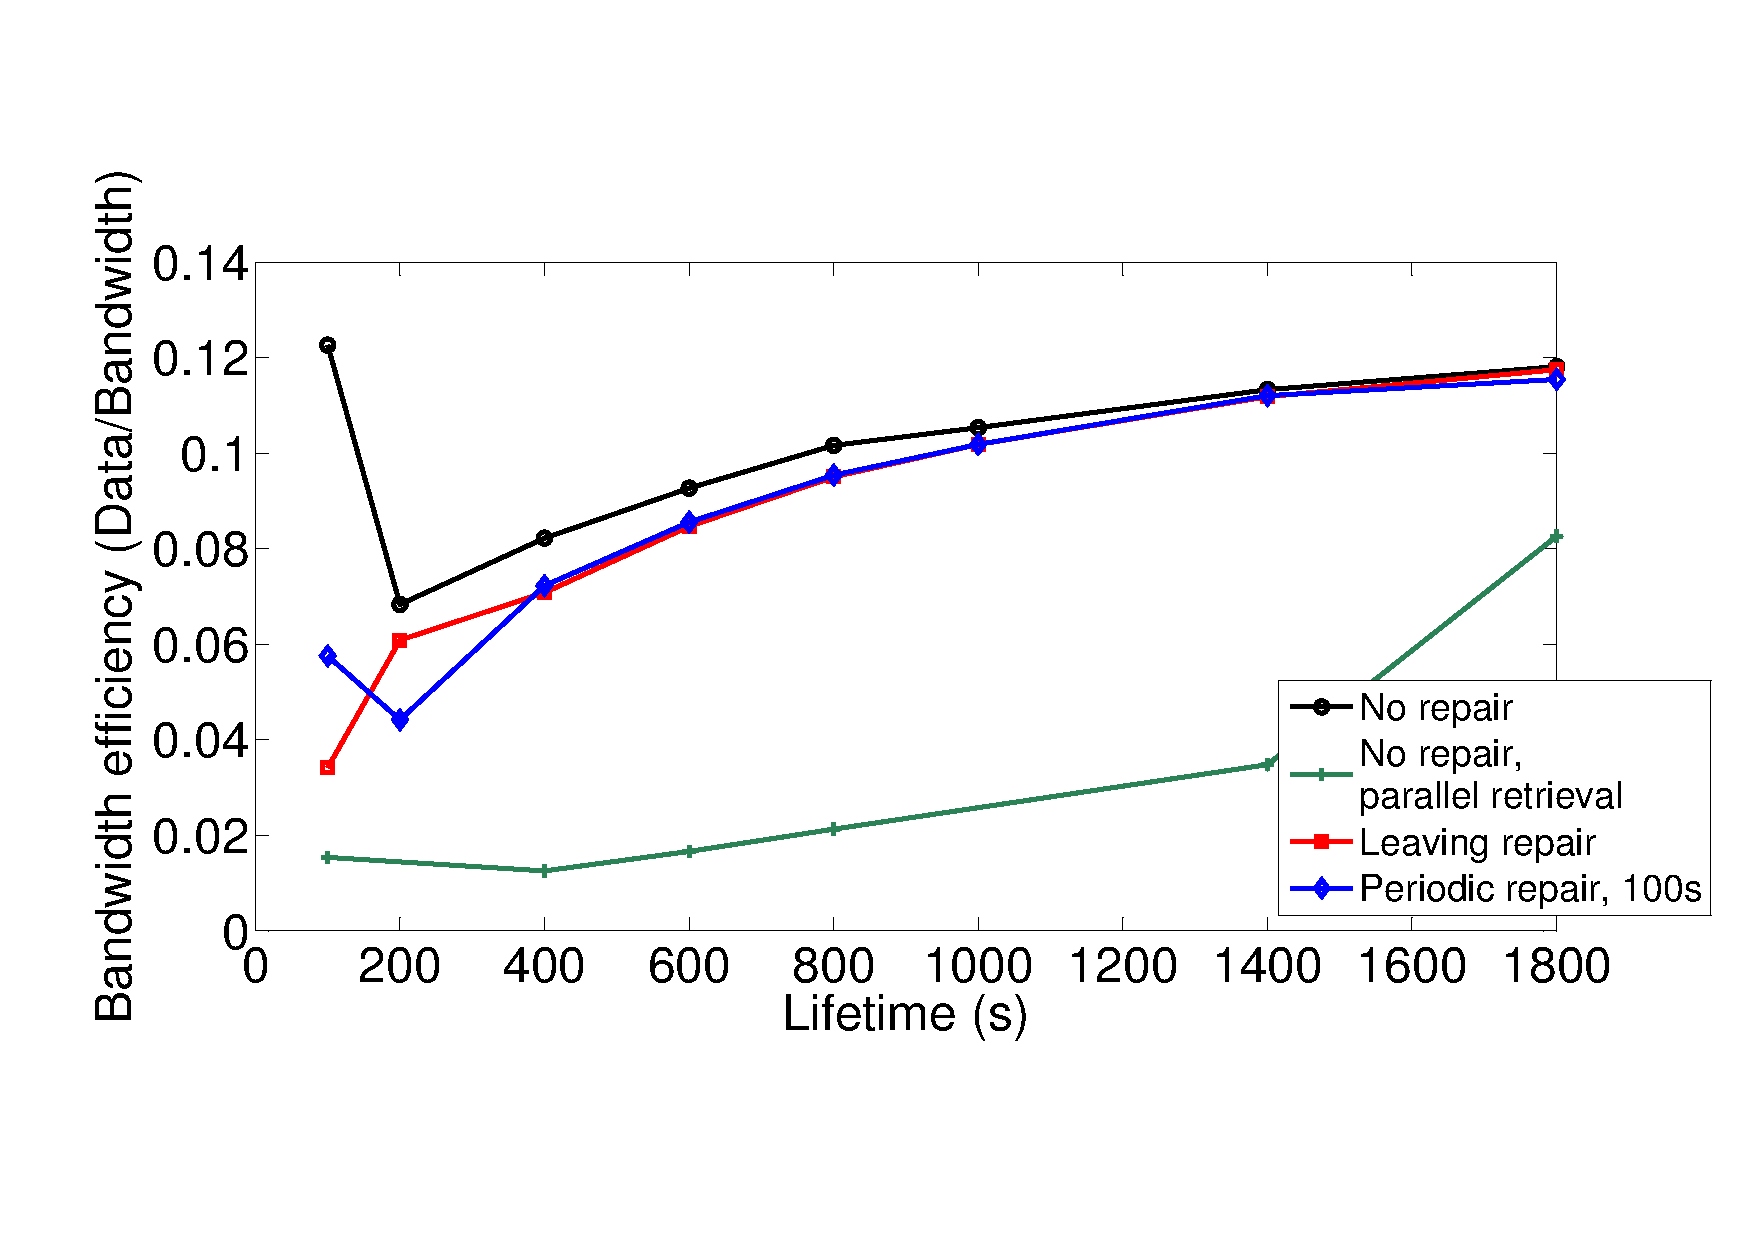
\includegraphics[clip=true, viewport=15mm 30mm 275mm 180mm, width=\columnwidth]{repair_bw_eff}
 \caption{Bandwidth efficiency of Pithos for various node lifetimes, comparing no repair, no repair with parallel retrieval, leaving repair and periodic repair with 100s periods.}
 \label{fig_repair_bw_eff}
\end{figure}
%
Figure \ref{fig_repair_bw_eff} compares the bandwidth efficiency of the various repair techniques. Bandwidth efficiency is defined to be the factor of usable data that would have been transferred to the higher layer, had the system been 100\% reliable, compared to the total bandwidth used by Pithos. 100\% reliability is used, otherwise bandwidth efficiency is also a function of reliability, since less data is transferred if fewer requests are successful. It should be noted that the largest part of Pithos's bandwidth usage is contributed by overlay storage, as shown in Sections \ref{overlay_results} and \ref{group_probability_bandwidth}.

Although parallel retrieval was shown to be the most reliable retrieval mechanisms for various node lifetimes, Figure \ref{fig_repair_bw_eff} shows that it is also the most bandwidth inefficient, with only between 1.5\% to 8\% usable data transferred. The bandwidth efficiency of leaving and periodic repair are similar for long peer lifetimes, compared to the periodic repair timer.

Bandwidth efficiency is monotonously increasing, because as peers remain in the network for longer periods of time, less bandwidth is required to repair missing replicas. Bandwidth efficiency also increases, since there is more usable data transferred when peers are alive for longer periods of time. Peers that live longer have less time to generate usable data. The increase in usable data for longer node lifetimes, than the object TTL does not lead to a significant increase in Pithos bandwidth.

Although doing no repair is less reliable, it is more bandwidth efficient, because no object repairs have to be performed.

\subsection{Conclusion}

The leaving and periodic repair mechanisms were found to posses similar reliability and bandwidth performances. It seemed that leaving repair does, however, cope better with dynamic node lifetimes. A periodic timer also has to be designed for specific network parameters, including expected node lifetime and object TTL. If, during the lifetime of the network, the parameters change, the system will not be able to dynamically adapt.

As expected, doing no repair is less reliable than doing repair, but uses less bandwidth. Parallel retrieval is highly reliable, but requires a large amount of bandwidth.

\section{Conclusion}

This section initially showed the storage and retrieval performance of Pithos, without taking into account group probability, object repair or malicious nodes. Fast storage was found to be sufficiently reliable for the large responsiveness gain it added. It was found that parallel storage are both more responsive and reliable than fast storage at the cost of additional bandwidth.

Overlay storage was found to be less reliable than initially thought, when taking into account its required bandwidth. Overlay storage is, however, the only way in which a peer may acquire data from outside of its group.

The responsiveness distributions for Pithos were also presented, along with a discussion of the results. The distributions verified the methods used to implement the store and retrieve mechanisms and also showed how the underlying group and overlay storage modules relate to the overall storage performance.

It was discussed that it is important to take group probability into account when evaluating Pithos performance. By varying the group probability, it was shown that the overall performance is a weighted average of the underlying group and overlay performances.

Tt was shown that all peers in Pithos are required to contribute storage space to the network.

The effect of repair was shown by evaluating Pithos for various repair methods with varying node lifetimes. It was found that repair significantly increases reliability when the expected node lifetimes are small, compared to the object TTL. Repair is not required, if node lifetimes are large, compared to the object TTL.

From the evaluation of object repair, it was found that there are many factors that influence how retrieval reliability. On a basic level, retrieval reliability is directly proportional to object lifetime. From the results shown, it was found that object lifetime is, therefore, related to node lifetimes, repair rates and object TTL.

It should be possible to design a storage system with predictable levels of reliability, to ensure correct functionality of the larger system that uses the storage system. It is, therefore, of benefit to be able to predict objects lifetimes in a distributed storage system. Of greater benefit is to be able to design a storage system to ensure required levels of expected object lifetimes. This is the focus of the next chapter. Predicting object lifetimes in finite network under churn.
